\section{Vortex formation at planetary gap edges in layered
  discs}\label{disc-planet} 
The previous simulations, while necessary to isolate the effect of 
viscosity on the linear RWI, has the disadvantage that the radially
structured viscosity profile may act to source radial disc structure
in the non-linear regime. In this section, we use disc-planet interaction to
create the disc structure required for instability, and employ a radially smooth
viscosity profile. We therefore expect viscosity to only
act as a damping mechanism. %This experiment separates out the cause of
%radial structure and 

%Gaps opened by giant planets in protoplanetary discs is a potential
%site for  he RWI. 
Vortex formation at gap edges is seen in many  
2D and 3D hydrdynamical simulations of giant planets in low viscosity discs 
\citep{valborro07,lin10,lin11a,lin12}. The fact that this is due to
the RWI has been explicitly verified through linear stability
analysis of planetary gap profiles produced from 2D simulations
\citep{valborro07,lin10}. Here, we simulate gap-opening giant planets
in 3D discs where the kinematic viscosity varies with height above the
disc midplane. Our numerical experiments are similar in spirit to
those performed by \cite{pierens10}, but our focus here is gap
stability in a layered disc. 
 
%In this case the required structure for instability, the PV extremum, 
%is induced by disc-planet interaction (cf. as an initial condition considered in the
%previous section). 

%We initialise a smooth disc ($A=1$ so there is no initial bump). The associated viscous timescale
%$t_\nu=r^2/\nu\sim 10^3P_0$ (for $\hat{\nu}\sim 10^{-4}$) is much
%longer than our simulation timescale. It is not crucial to initialize
%the simulation with an exact steady state since the giant planet
%maintains the gap. We therefore employ a simpler viscosity profile than
%the previous experiment.   

%no initial pert

\subsection{Radially smooth viscosity profile for disc-planet
  interaction}\label{planet_visc_mode} 
Using the same notation as \S\ref{visc_model}, we impose a viscosity
profile $\hat{\nu}$ such that 
\begin{align}\label{planet_visc_profile}
  \hat{\nu}\Sigma_i(R)\frac{d\ln{\Omega_i}}{d\ln{R}} =
  \hat{\nu}_0\left[1+Q(\psi)\right]\Sigma_i(r_0)\left.\frac{d\ln{\Omega_i}}{d\ln{R}}\right|_{r_0}.      
\end{align}
We have set the dimensionless argument in Eq. \ref{step} to
$\zeta=\psi$. Recall $\psi=\pi/2-\theta$ is the angular height away from the midplane. 
The viscosity increases from its floor value $\hat{\nu}_0$ by a factor
$A_\nu$ for $\psi > \zeta_\nu$. So the viscous layer is 
a wedge in the meridional plane, which conveniently fits into our
spherical grid. Note that setting $\psi = 0$ in Eq. \ref{planet_visc_profile} gives
the appropriate viscosity profile for a razor-thin viscous disc in
steady state when the initial cylindrical radial velocity 
is set by Eq. \ref{init_vr}. 

The typical viscosity value adopted for disc-planet simulations, 
$\hat{\nu}\sim 10^{-5}$ or $\alpha\sim 10^{-3}$, is known to surpress
vortex formation in 2D \citep{valborro07, mudryk09}. 
We therefore choose a floor viscosity of $\hat{\nu}_0=10^{-6}$.
The angluar thickness of the viscosity transition is fixed to
$\Delta\zeta_\nu = 0.2h$. Fig. \ref{planet_visc2d} gives an example of this
viscosity profile. We will quote the thickness of the viscous layer as a 
percentage of the entire $\theta$ domain size. 

\begin{figure}
  \centering
  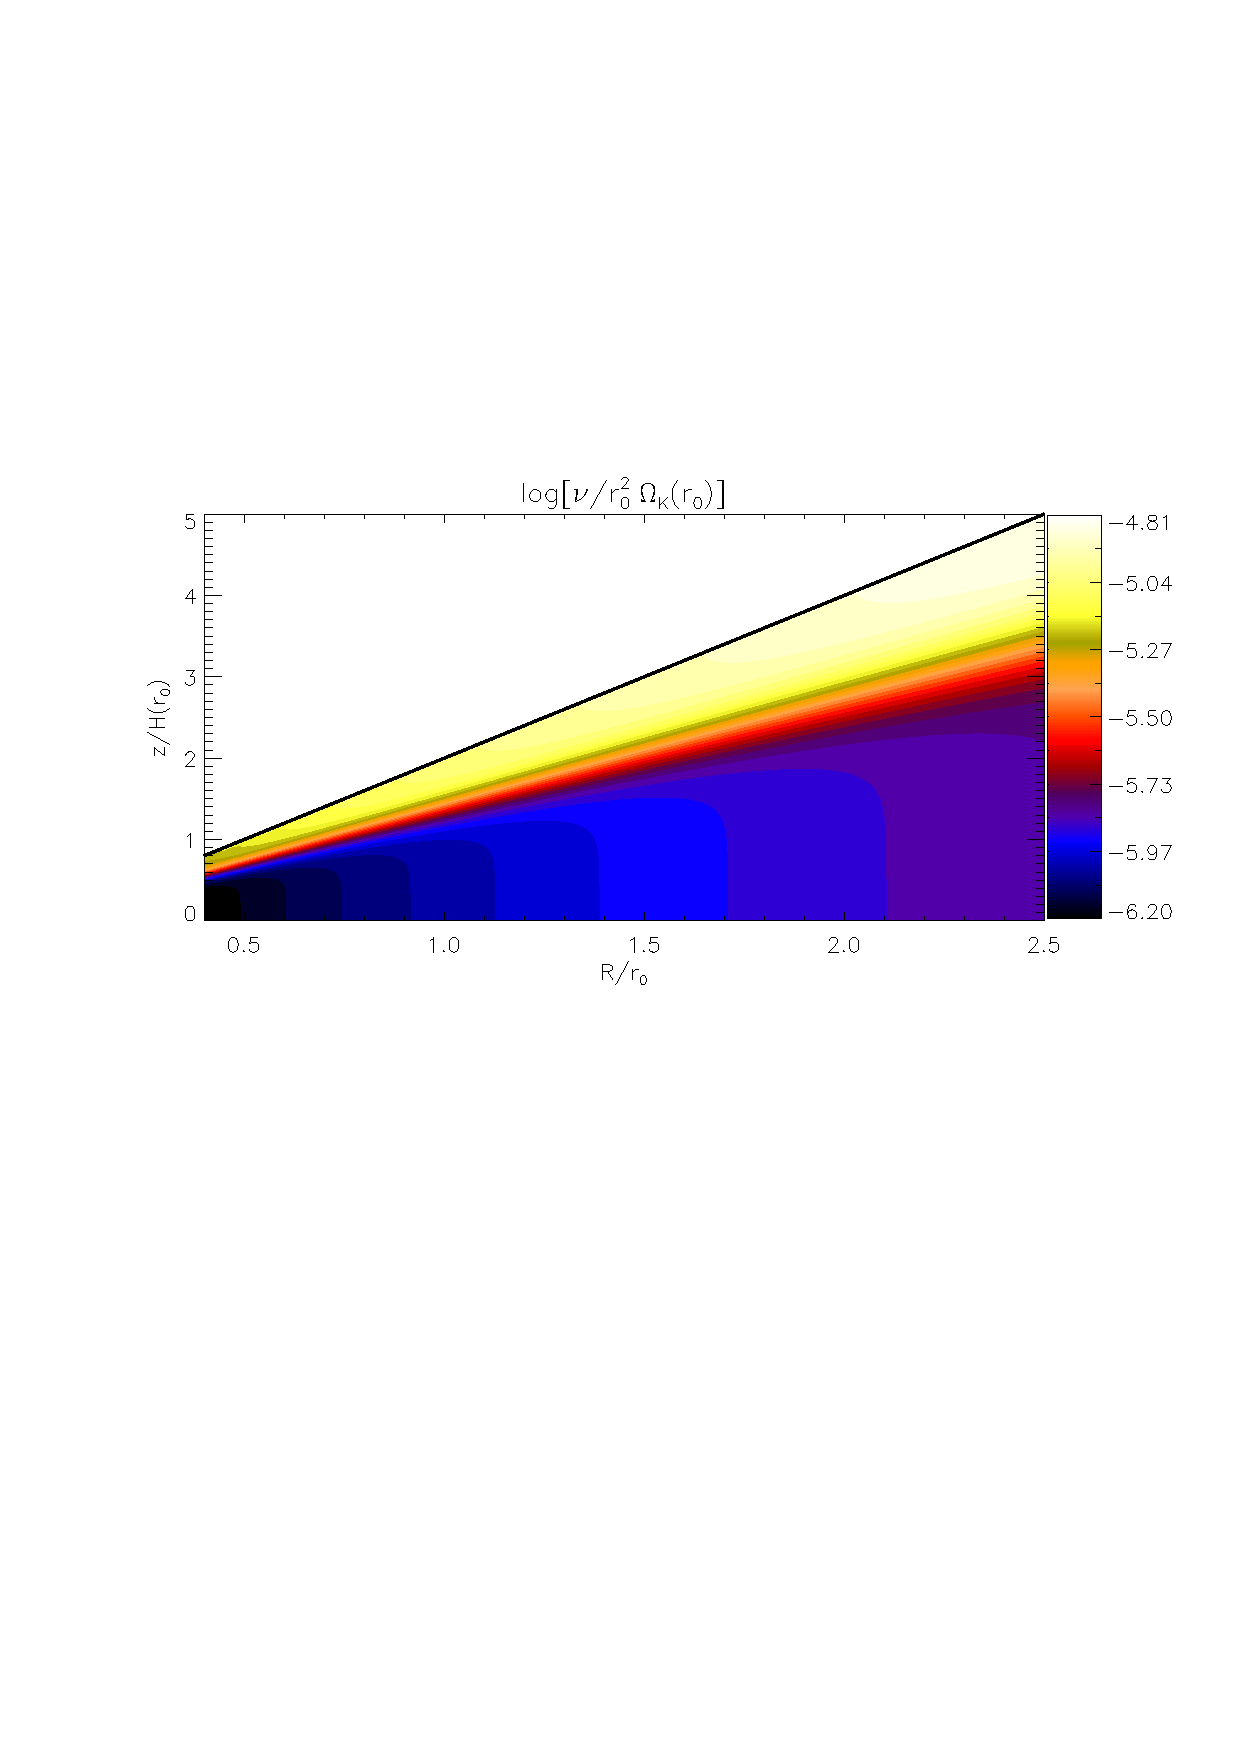
\includegraphics[width=\linewidth]{figures/pdisk_visc2d_planet}
  \caption{Example of the `wedge' viscosity profile
    imposed in disc-planet simulations (Eq. \ref{planet_visc_profile}). This specific plot
    corresponds to case P1. The solid line
    delineates the upper boundary of the computational domain.
    \label{planet_visc2d}}
\end{figure}

%This viscosity profile is a smooth
%function of radius, meaning a localized radial density structure will
%be smoothed out, unless it is maintained by an external
%source (the planet in our case). We therefore expect viscosity to only
%act as a damping mechanism, c.f. a source for radial structure in the
%previous section. 

\subsection{Disc-planet simulations} 
We simulate discs with $h=0.05$ and radial extent
$[\rin,\rout]=[0.4,2.5]r_0$. Initially the surface density is smooth
($A=1$) with cylindrical radial velocity is given by
Eq. \ref{init_vr}. The standard resolution is $(N_r, N_\theta,
N_\phi)=(256, 32n_h, 768)$, corresponding to $6,\,32,\,6$ 
cells per $H$ along the $r,\theta,\phi$ directions at the reference
radius.  

We insert into the disc a planet of mass  
$M_p=10^{-3}M_*$, which corresponds to a Jupiter mass planet if
$M_*=M_{\sun}$. The softening length adopted for the planet potential is
$\epsilon_p=0.5r_h$. The planet potential is switched on 
smoothly over $t\in[0,10]P_0$. We note that the disc can be considered
as two-dimensional for gap-opening giant planets, because the Hill
radius $r_h$ exceeds the local scale-height $H_0$ ($r_h/H_0\simeq1.4$
in our cases).   

We remark that the above choice of physical and numerical parameter
values are typical for global disc-planet simulations
\citep[e.g.][]{valborro06,mignone12}.   

\subsubsection{Standard runs} 
The fiducial vertical extent of our disc model is $n_h=2$
scale-heights at $R=r_0$.  The control run, case P0, has $A_\nu=1$ so there is 
no viscous layer. The kinematic viscosity is therefore
$\hat{\nu}\sim10^{-6}$  everywhere. We then introduce a viscous
layer (or wedge) occupying the uppermost $25\%$ and $50\%$ of the
vertical domain in cases P1 and P2, by choosing the transition angle
at $\zeta_\nu = 1.5h,\,1.0h$, respectively. These layers have a kinematic 
viscosity of $\hat{\nu}\sim 10^{-5}$ by setting $A_\nu=10$.  (See
Fig. \ref{planet_visc2d} for the viscosity profile for case P1.)  

%For completeness we also performed two high-viscosity simluations
%which do not develop vortices. Case P3 has $\hat{\nu}\sim10^{-5}$
%throughout the vertical extent, while in case P4 the uppermost $25\%$
%of the vertical domain has $\hat{\nu}\sim10^{-4}$. The purpose is to
%examine how a stable gap profile is affected by layered viscosity. 

\subsubsection{Extended vertical domain}
We also consider two runs with an extended vertical domain size
$n_h=3$. Case P3 has $A_\nu=1$ so there is no viscous layer. For case
P4 we set the transition angle $\zeta_\nu=2h$ with $A_\nu=100$. 
Thus, the viscous layer with $\hat{\nu}\sim10^{-4}$ occupies $33\%$ of
the uppermost vertical domain. %Note that most of the mass is contained
%in the low viscosity layer. 
%We also consider case P6 without a
%viscous layer but 


%%%%%%%%%%%%%%%%%%%%%%%%%%%%%%%%%%%%%%%%%%%%%%%%%%%%%%%%%%%%%%%%%%%%%%%%%%%%%%%


\subsection{Results}
Our disc-planet simulations are summarised in Table \ref{planet_sims}.
We focus on vortex-formation at the outer gap edge. 
The non-axisymmetric mode amplitude in the last column was 
averaged over the shell $r\in[1.2,1.6]r_0$ and over time 
$t\in[100,150]P_0$. We examine the $m=1$ mode since 
for non-self-gravitating planetary gaps, if unstable, usually develop
a single vortex in quasi-steady state \citep{valborro07,lin10}.   

%for  mode amp: spatial average over [1.2,1.6], time average over [100,150]P_0

\begin{table}
  \centering
  \caption{Summary of disc-planet simulations. These runs employ the
    `wedge' viscosity model described by
    Eq. \ref{planet_visc_profile}. The upper viscous layer is
    quoted as a fraction of the vertical domain at 
    $R=r_0$. \label{planet_sims}}  
    \begin{tabular}{lccccr}
      \hline\hline
      %      \multicolumn{6}{c}{\phantom{stuff}} &
      %      \multicolumn{3}{c}{Linear phase ($t\leq10P_0$)}&
      %      \multicolumn{3}{c}{$t=100P_0$}\\
      %      \cline{7-9}\cline{10-12}
      Case & $n_h$ & $A_\nu$ &$\zeta_\nu/h$ & visc. layer& $10^2\overline{a}_1$ \\ 
      \hline
      P0 &  2     &    1    &    n/a      & none     &   14.3    \\% Ro~ -0.03
      P1 &  2     &    10   &    1.5      & $25\%$  &    11.9     \\ 
      P2 &  2     &    10   &    1.0      & $50\%$  &    6.1      \\
%      P3 &  2     &    10   &    n/a      & none    &    ??      \\
%      P4&  2     &    100  &    1.5      & $25\%$  &    ??     \\
      P3 &  3     &    1    &     n/a      & none  &     18.3   \\
      P4 &  3     &    100   &    2.0      & $33\%$ &     3.5    \\
      \hline
  \end{tabular}
\end{table}

\subsection{Introducing a viscous layer}
We first compare cases P0, P1 and P2. Fig. \ref{planet_gap} 
shows that the PV profiles induced by the planet is very
similar. (In fact, case P0 and P1 already non-axisymmetric
disturbances at the chosen snapshot, but they are weak and is not
reflected in the azimuthally averaged PV plots.) This shows that gap
opening is not sensitive to the presence of a viscous layer.  

\begin{figure}
  \centering
  \includegraphics[width=\linewidth]{figures/pdisk_vorten1d_cases_002.ps}
  \caption{Potential vorticity perturbation in the disc-planet
    simulations P0, P1 and P2. The snapshot is taken 10 orbits after
    the planet is fully introduced. %% Both P0 and P1 already developed
    %% small non-axisymmetric
    \label{planet_gap}}
\end{figure}

Indeed, the density perturbations shown for $t=50P_0$ in
Fig. \ref{jup0} indicates that the RWI develops in all cases. This is
consistent with our previous experiments which show that the linear
instability is largely unaffected by viscous layers. However,   
the $t=50P_0$ snapshot shows that thickening the viscous layer does lead
to somewhat larger vortices, as expected because of viscous diffusion.   

On the other hand, a viscous layer can have significant influences  
well into the non-linear regime. Fig. \ref{jup0} shows that the vortex
merging proceeds in case P0 to form a single vortex at the outer gap
edge at $t=100P_0$. This is a standard result for giant planets in
low viscosity discs \citep{valborro06,valborro07}.  

The final vortex is weaker 
in case P1, as indicated by the $m=1$ amplitude in Table
\ref{planet_sims}. Most interestingly, the vortices are transient in case P2,
being absent after $t=100P_0$. This means that vortex formation can be
surpressed by viscous layers. This suggests that for long-term vortex
survival, the entire vertical extent of the disc should be `dead'. 

\begin{figure}
   \centering
   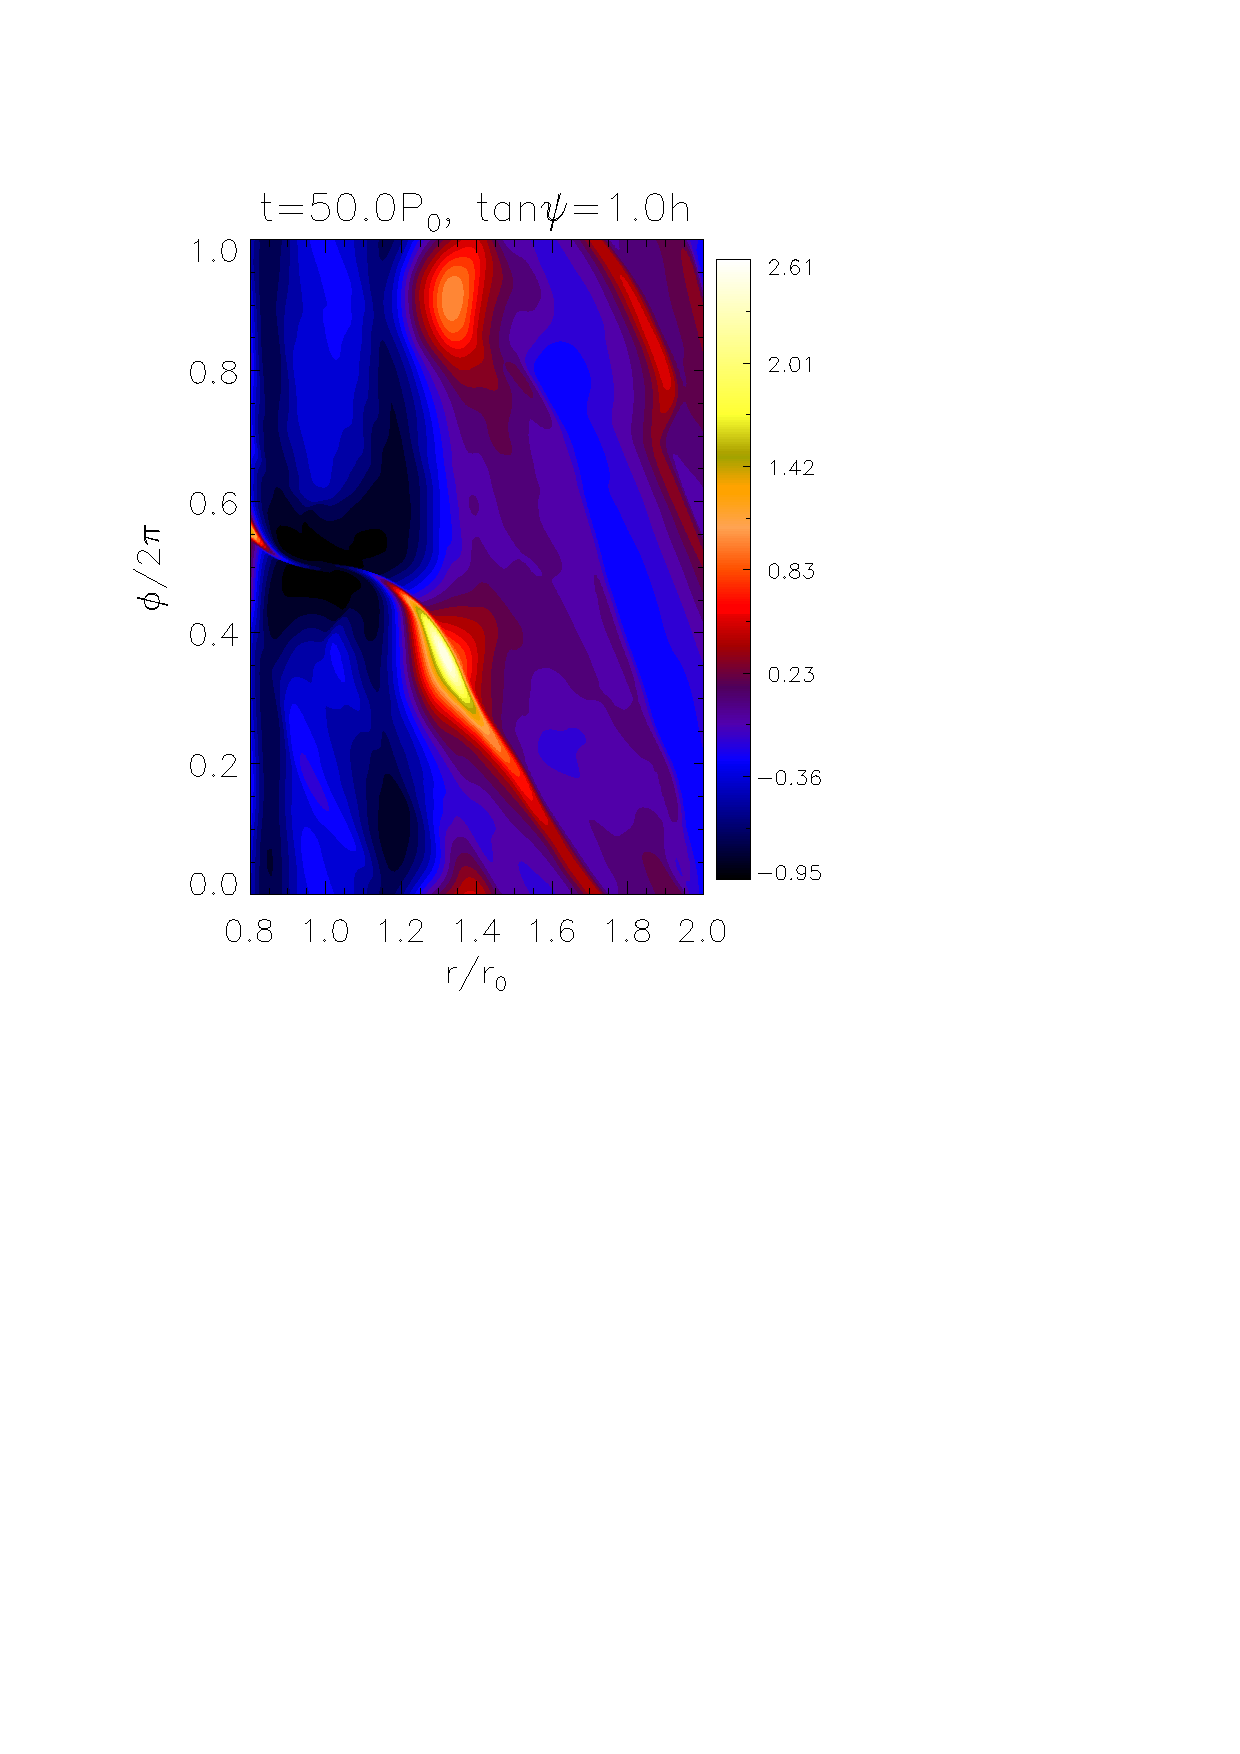
\includegraphics[scale=.39,clip=true,trim=0cm 1.84cm 0cm
     0cm]{figures/jup0_pdisk005}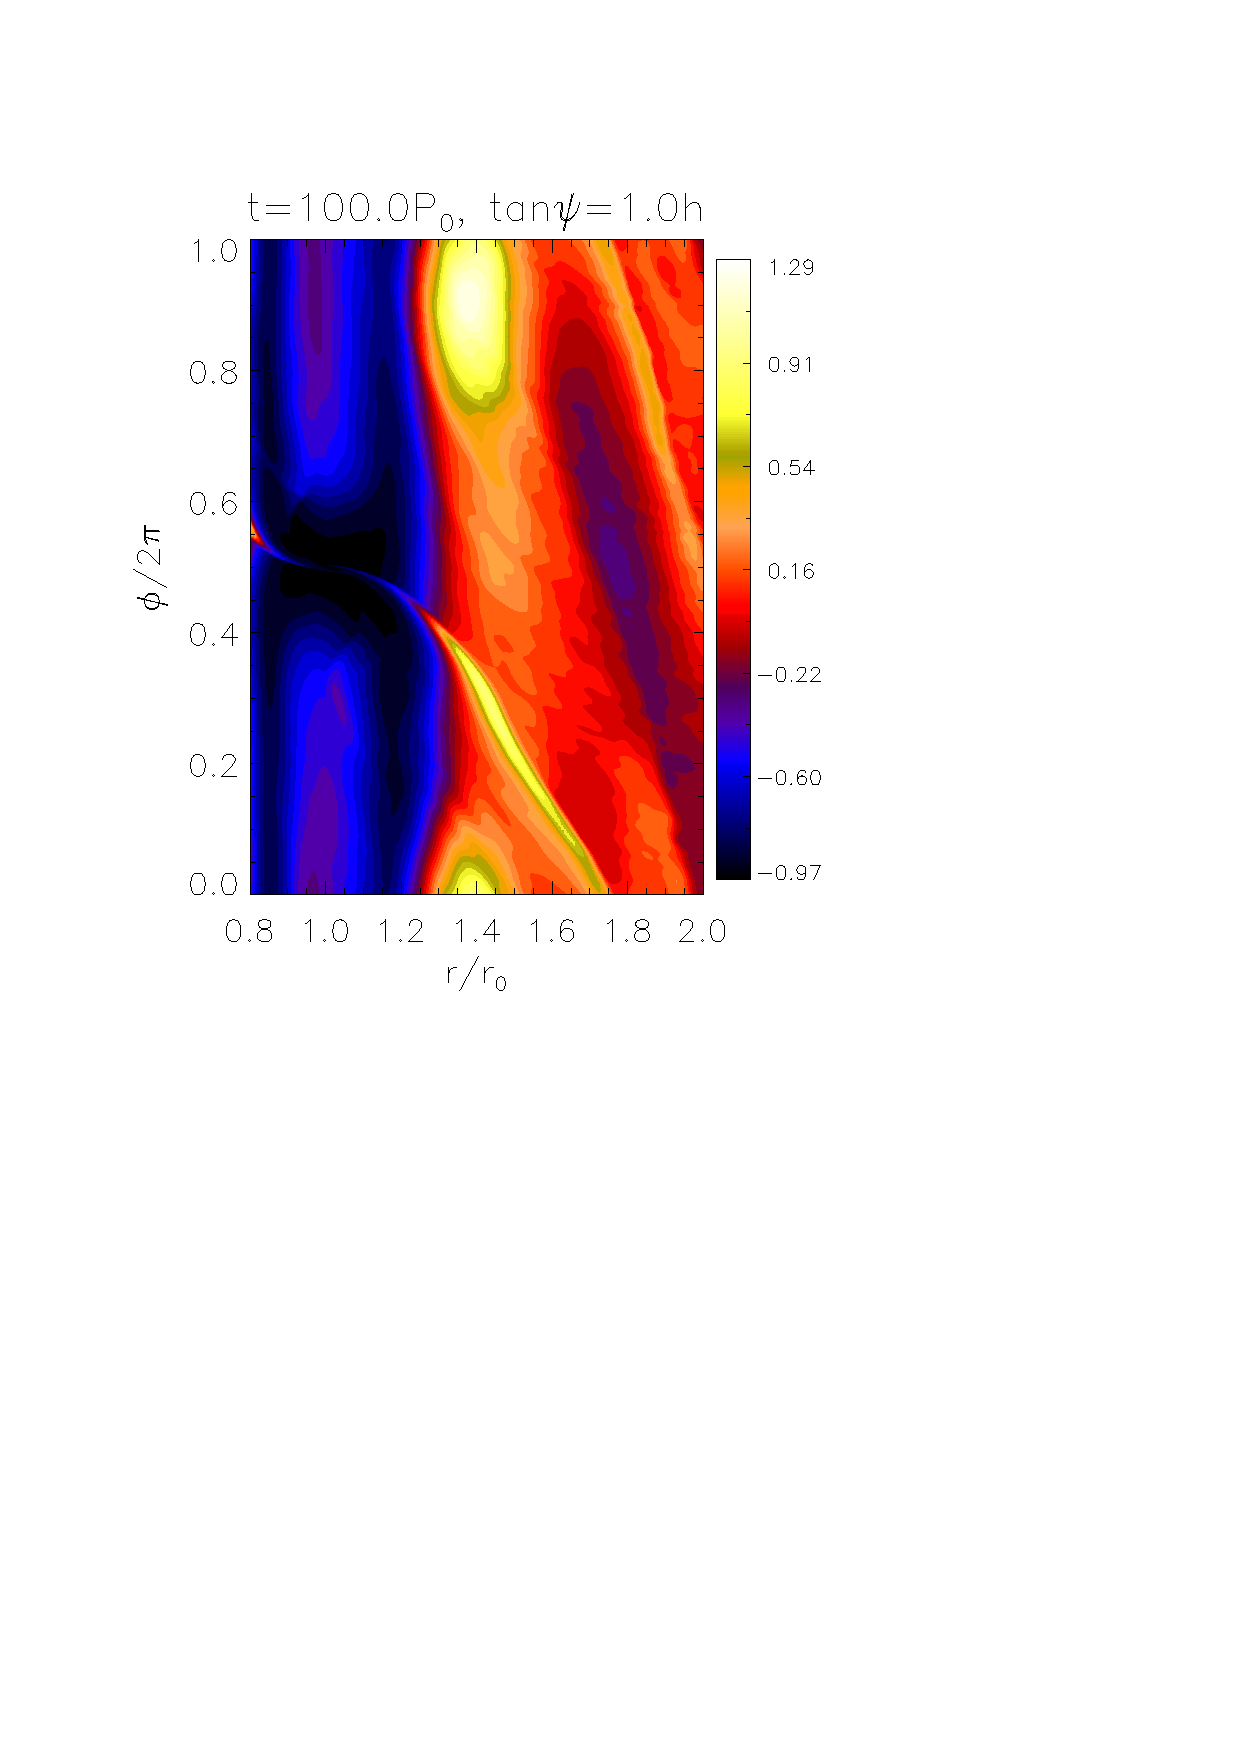
\includegraphics[scale=.39,clip=true,trim=2.3cm
     1.84cm 0cm
     0cm]{figures/jup0_pdisk010}\\%% 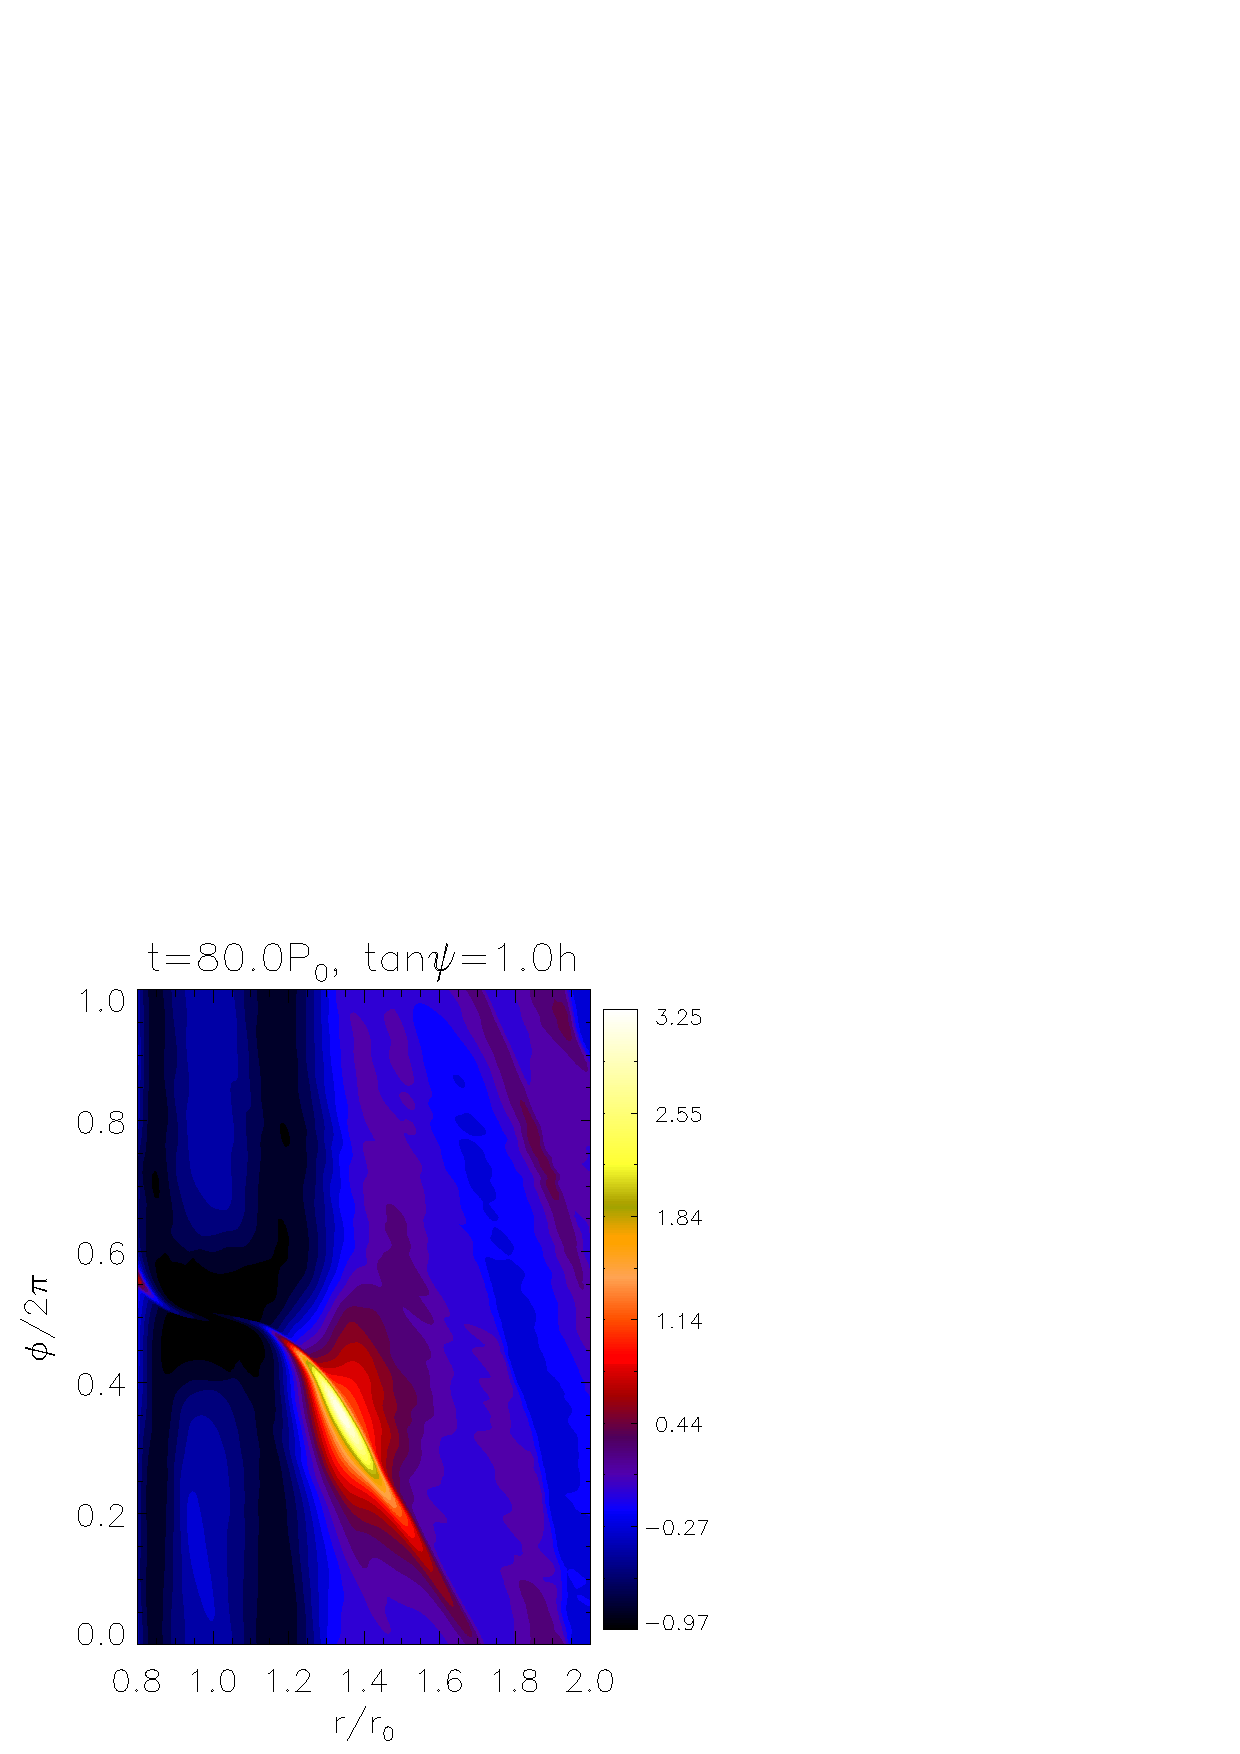
\includegraphics[scale=.27,clip=true,trim=2.3cm
     %% 1.84cm 0cm
     %% 0cm]{figures/jup0_pdisk008}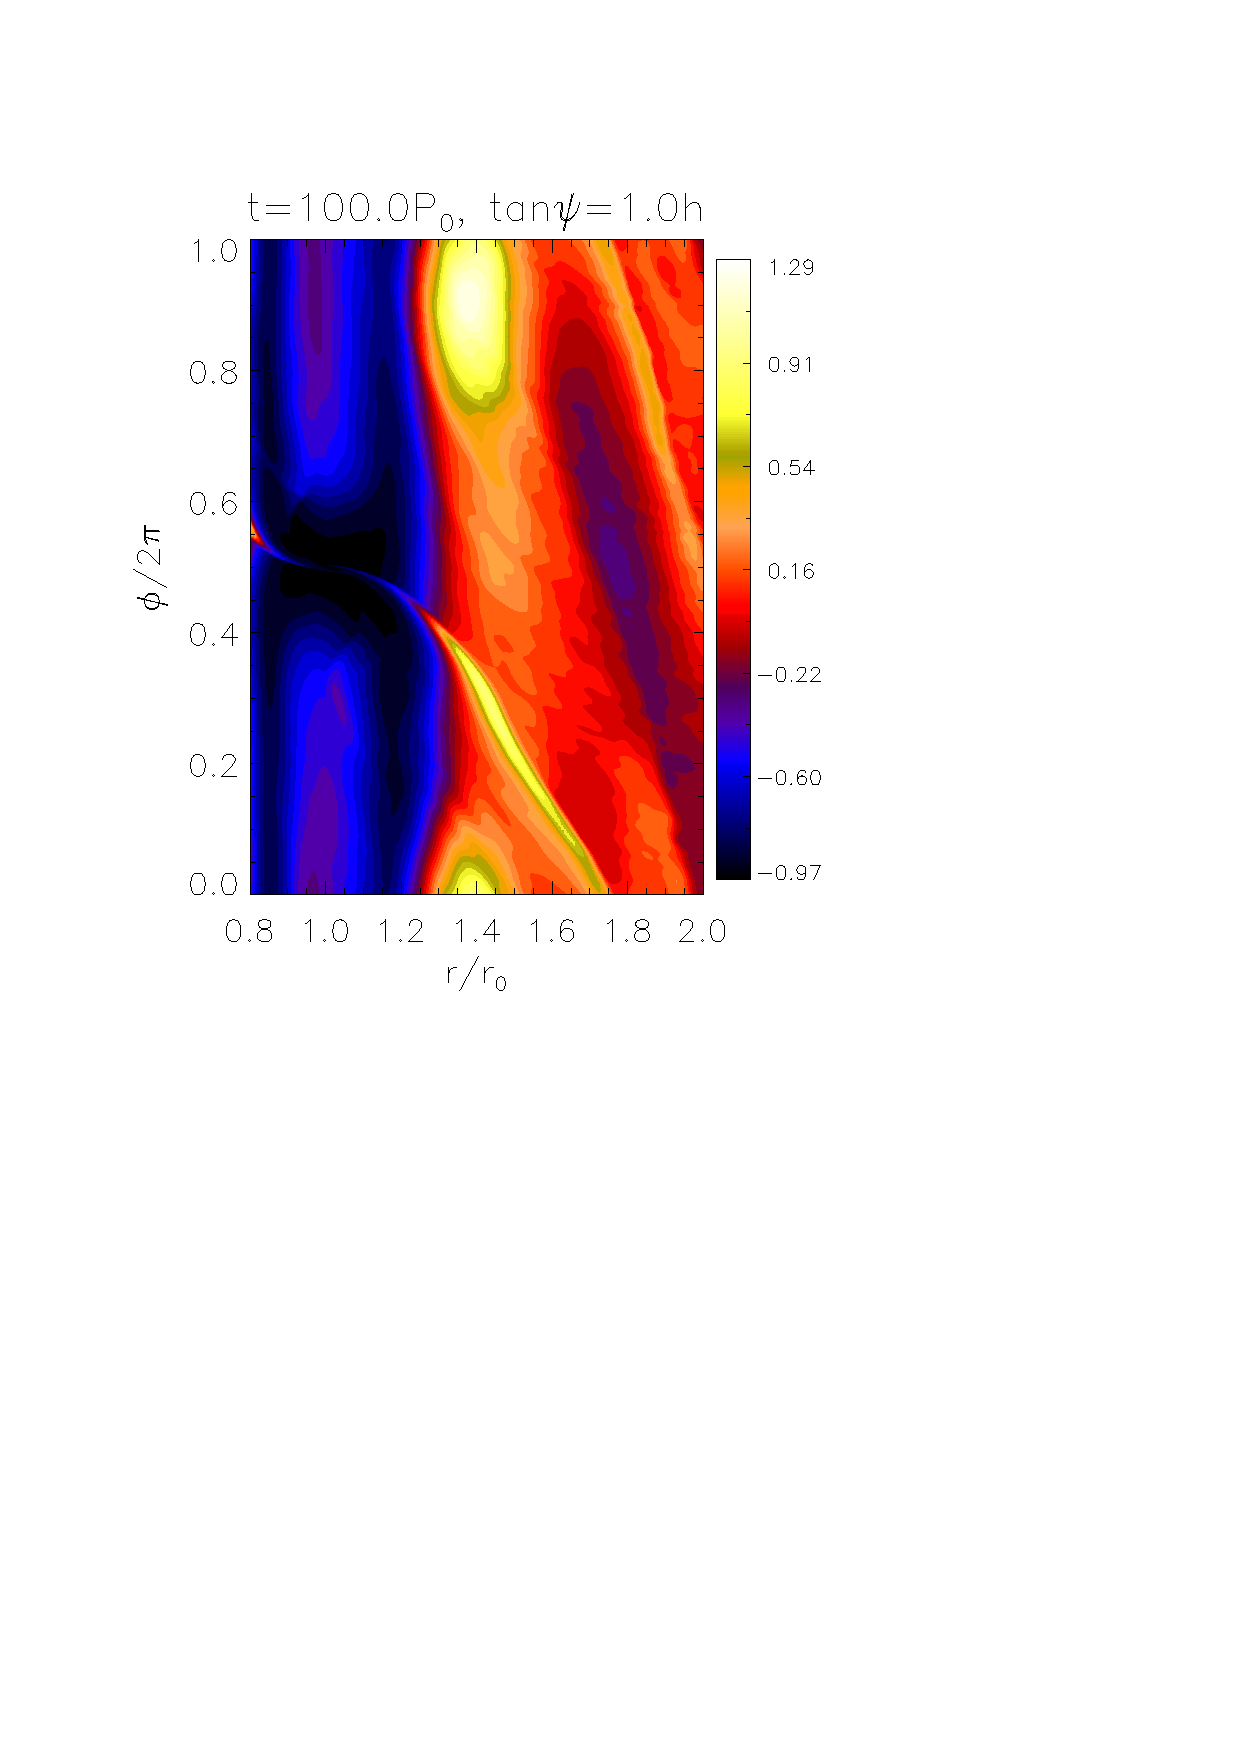
\includegraphics[scale=.27,clip=true,trim=2.3cm
     %% 1.84cm 0cm
     %% 0cm]{figures/jup0_pdisk010}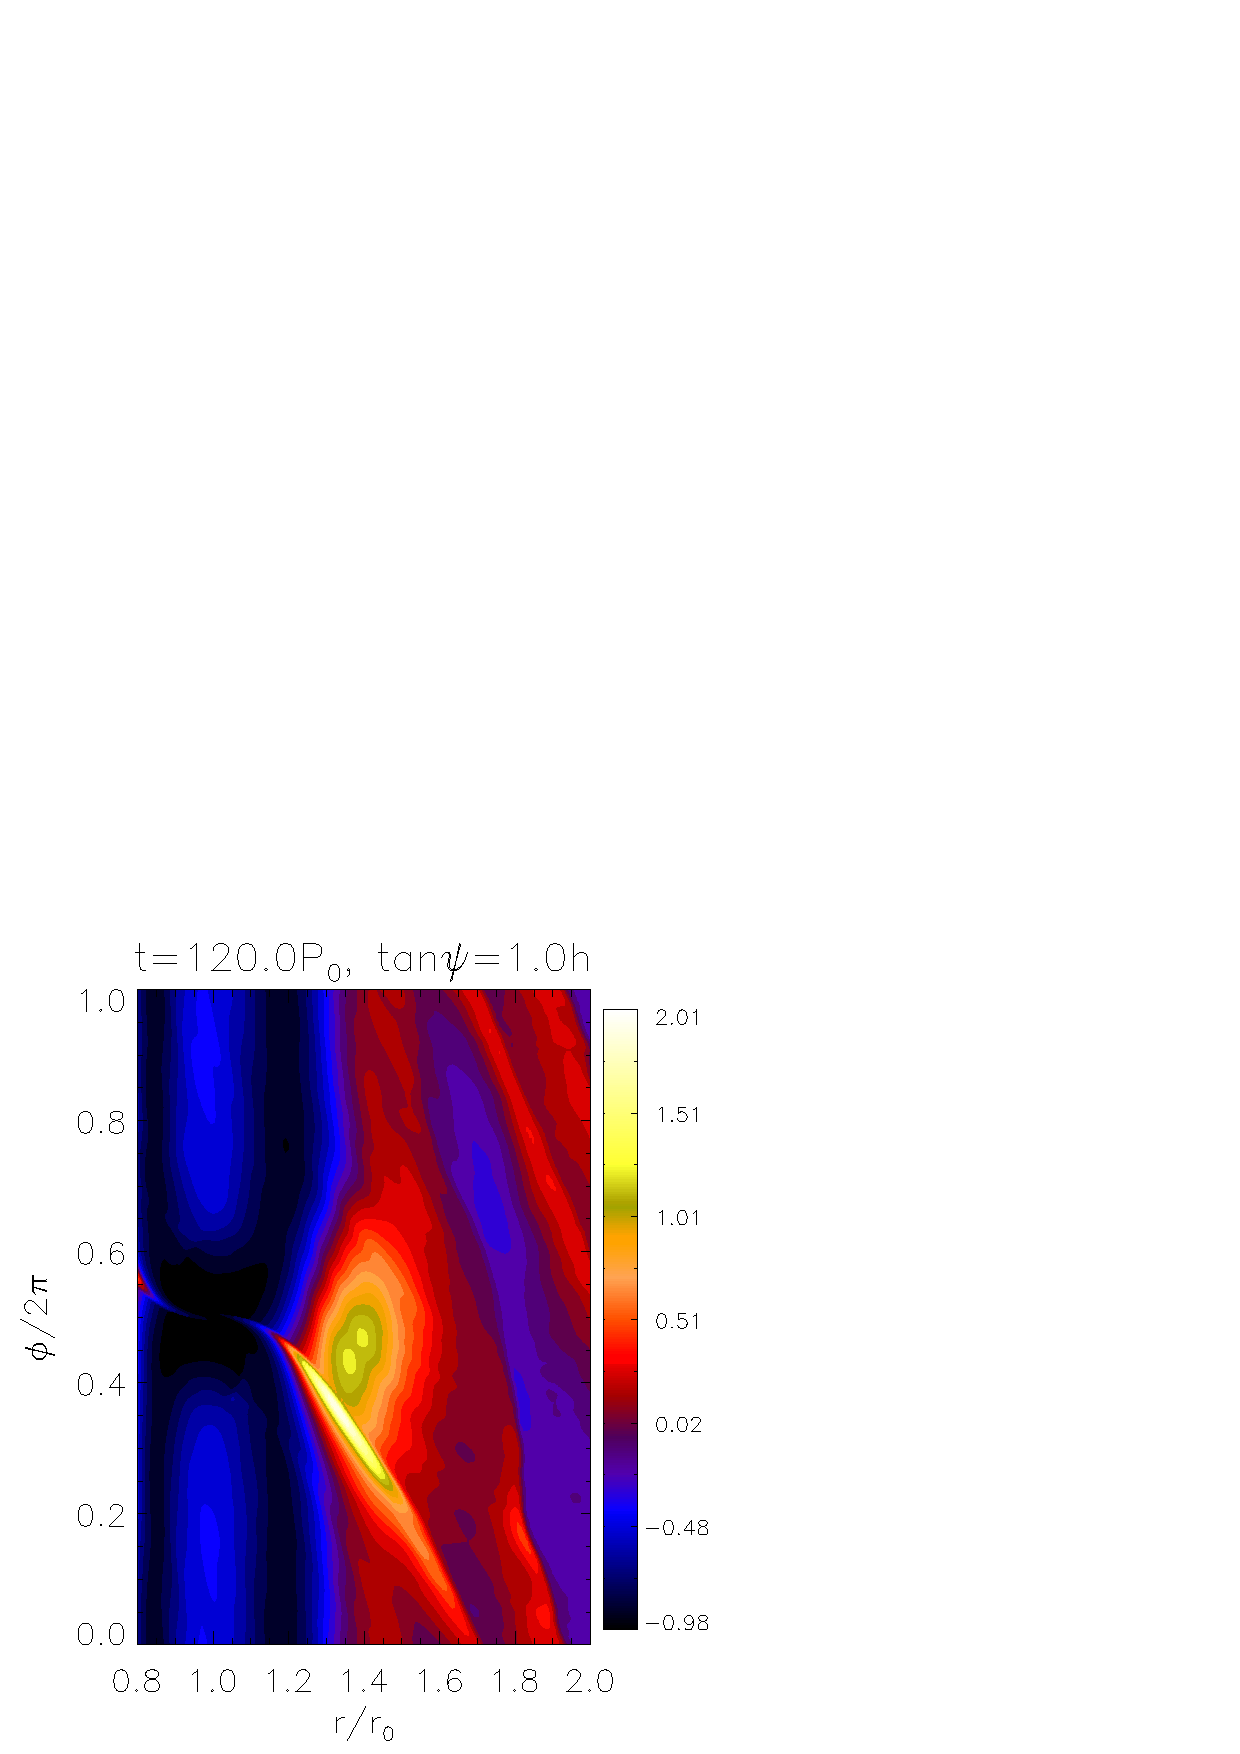
\includegraphics[scale=.27,clip=true,trim=2.3cm
     %% 1.84cm 0cm
     %% 0cm]{figures/jup0_pdisk012}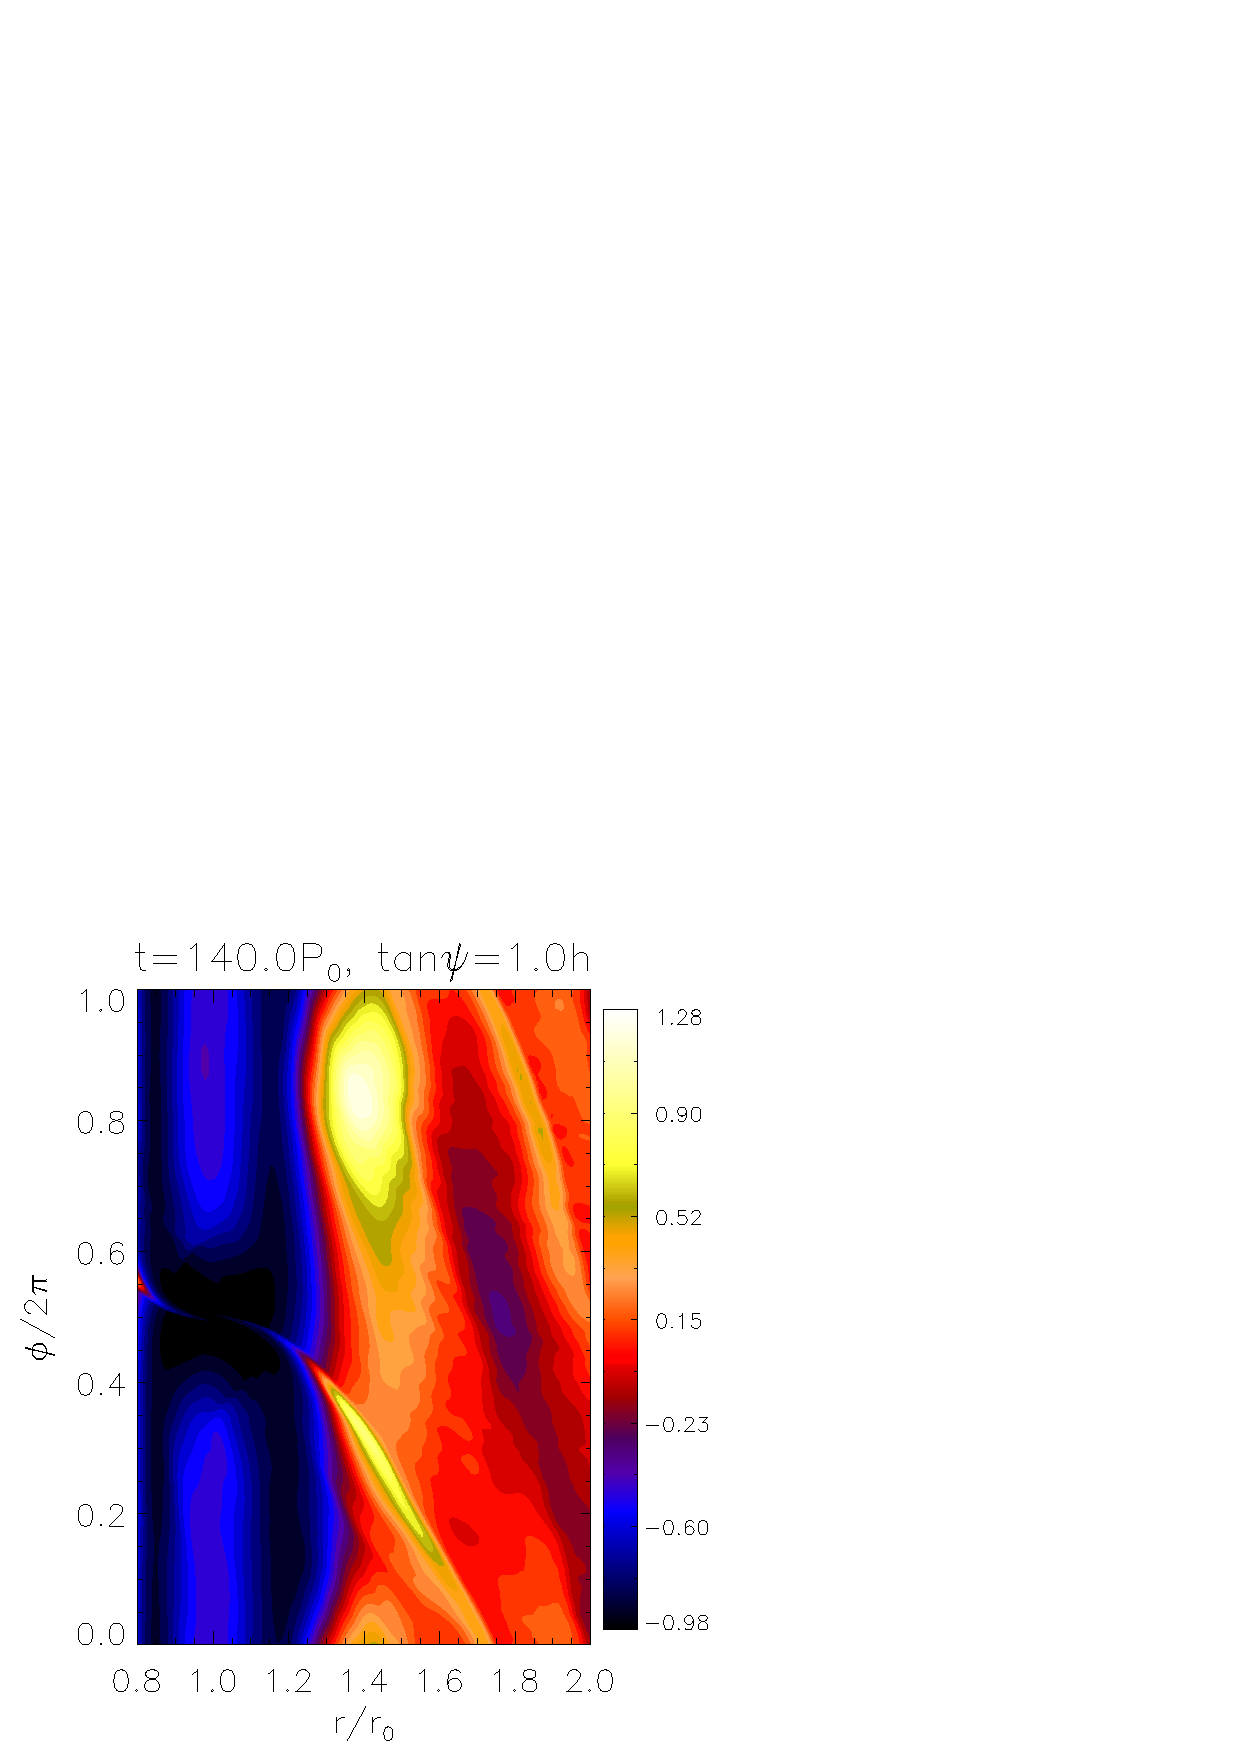
\includegraphics[scale=.27,clip=true,clip=true,trim=2.3cm 
     %% 1.84cm 0cm
     %% 0cm]{figures/jup0_pdisk014}\\
   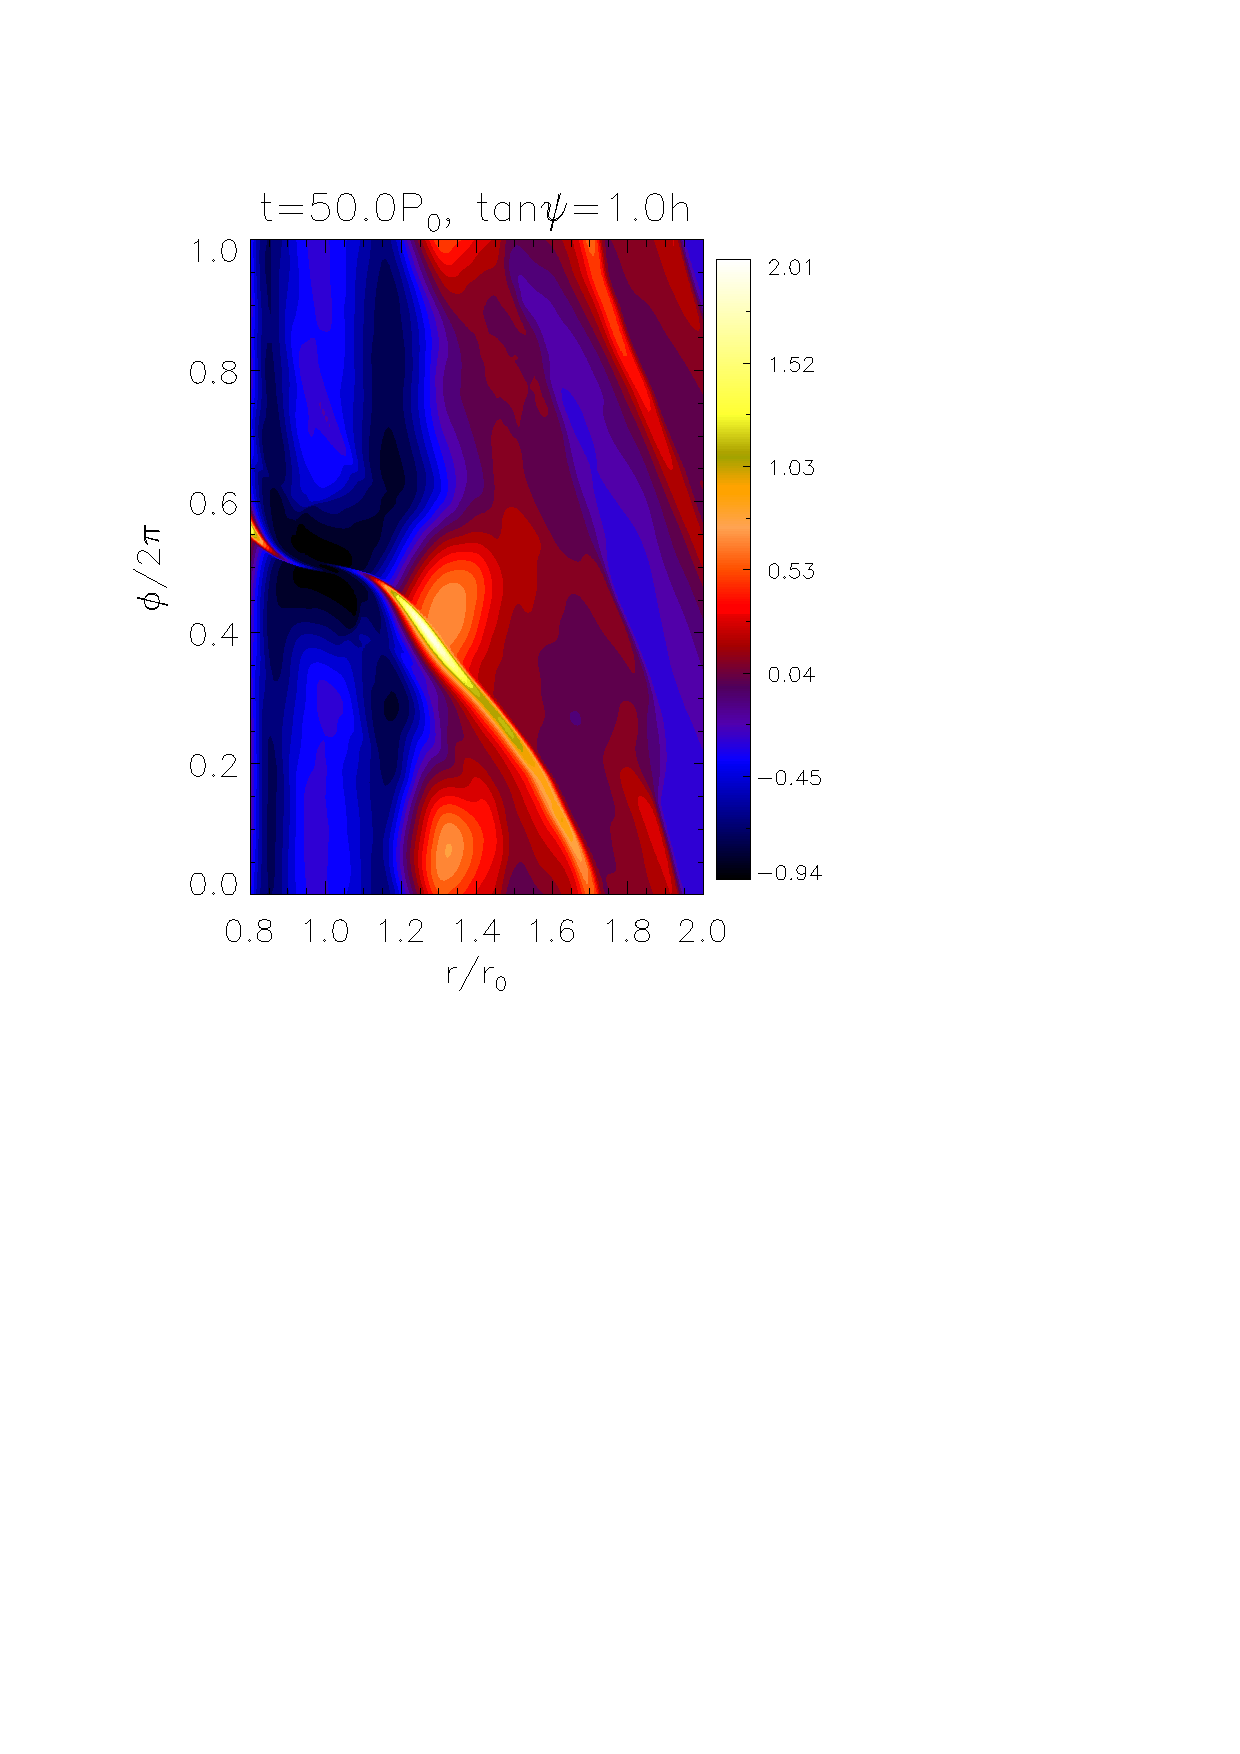
\includegraphics[scale=.39,clip=true,trim=0cm 1.84cm 0.0cm
     0.99cm]{figures/jup2_nuamp10_pdisk005}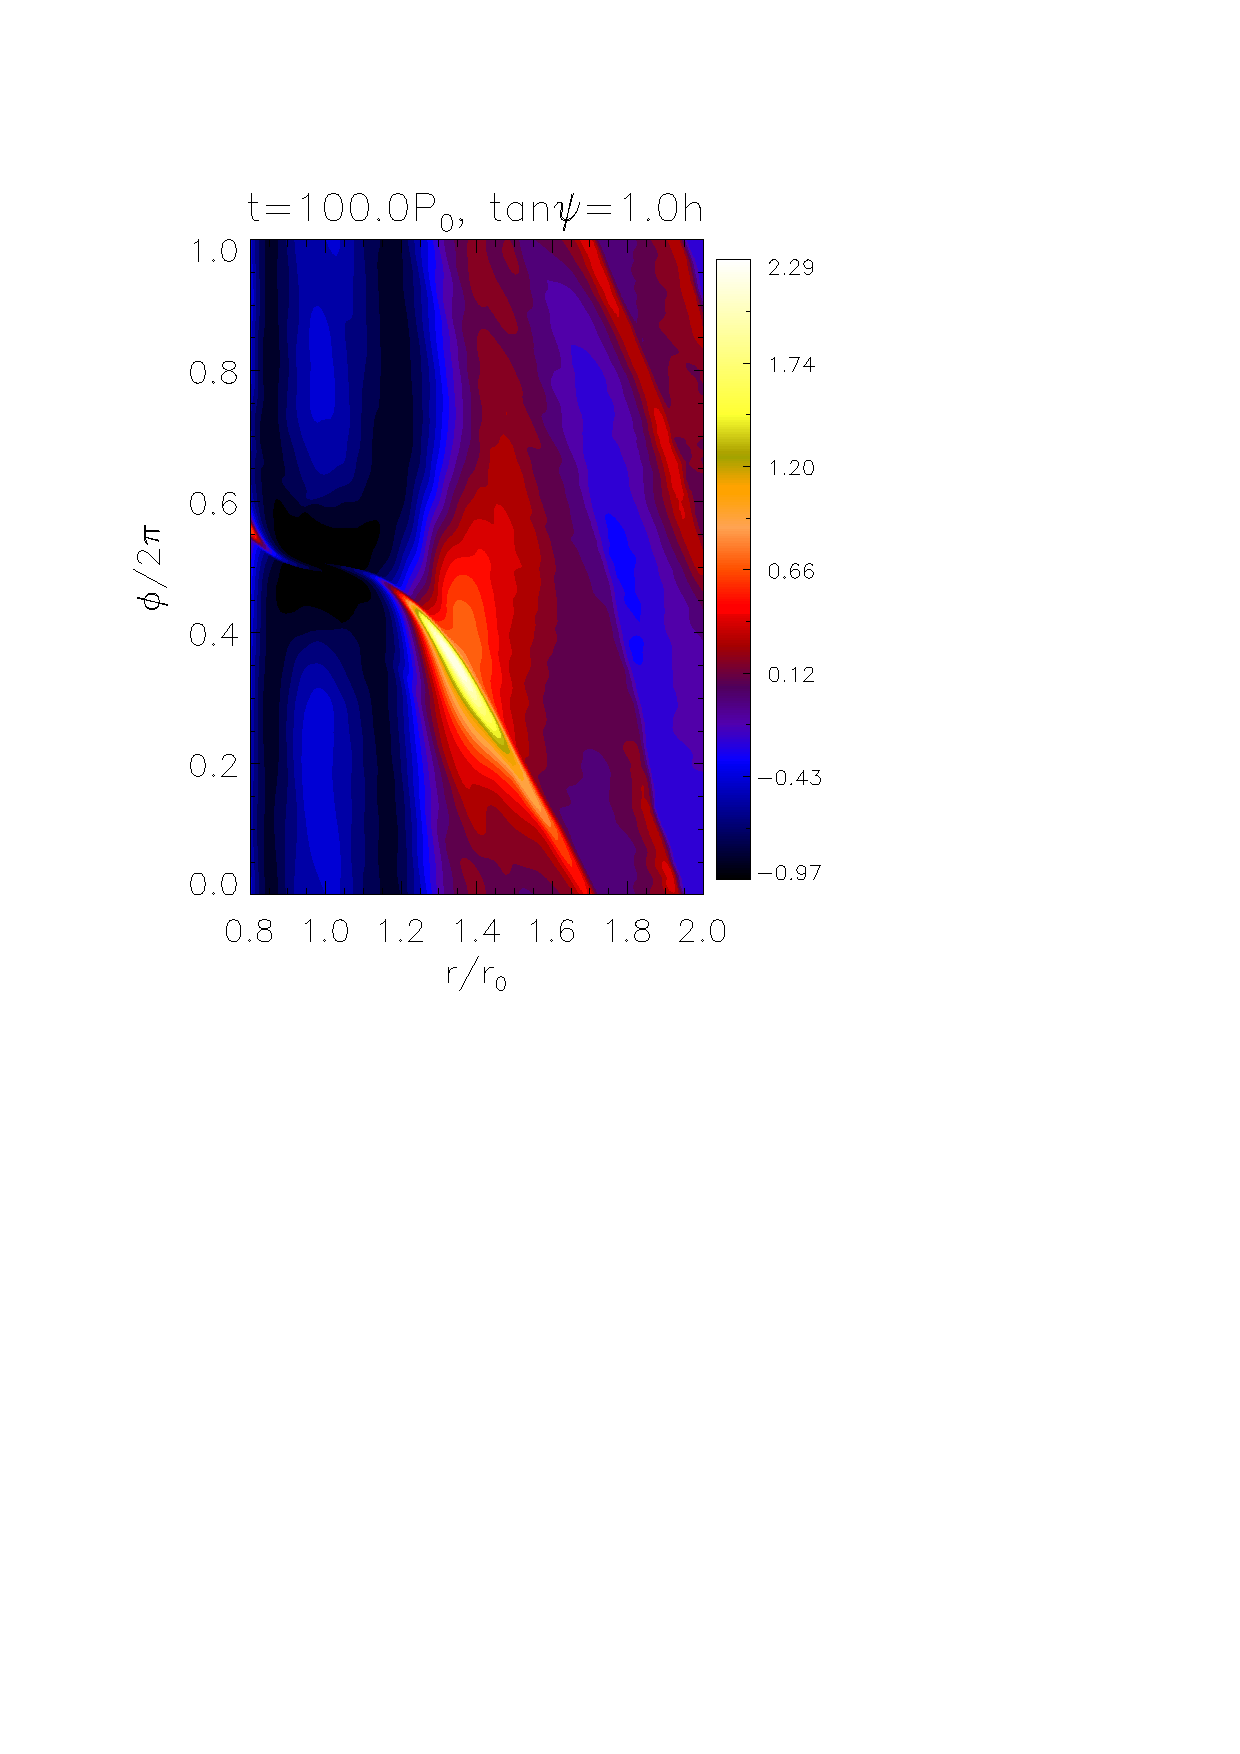
\includegraphics[scale=.39,clip=true,trim=2.3cm
     1.84cm 0.cm
     0.99cm]{figures/jup2_nuamp10_pdisk010}\\%% 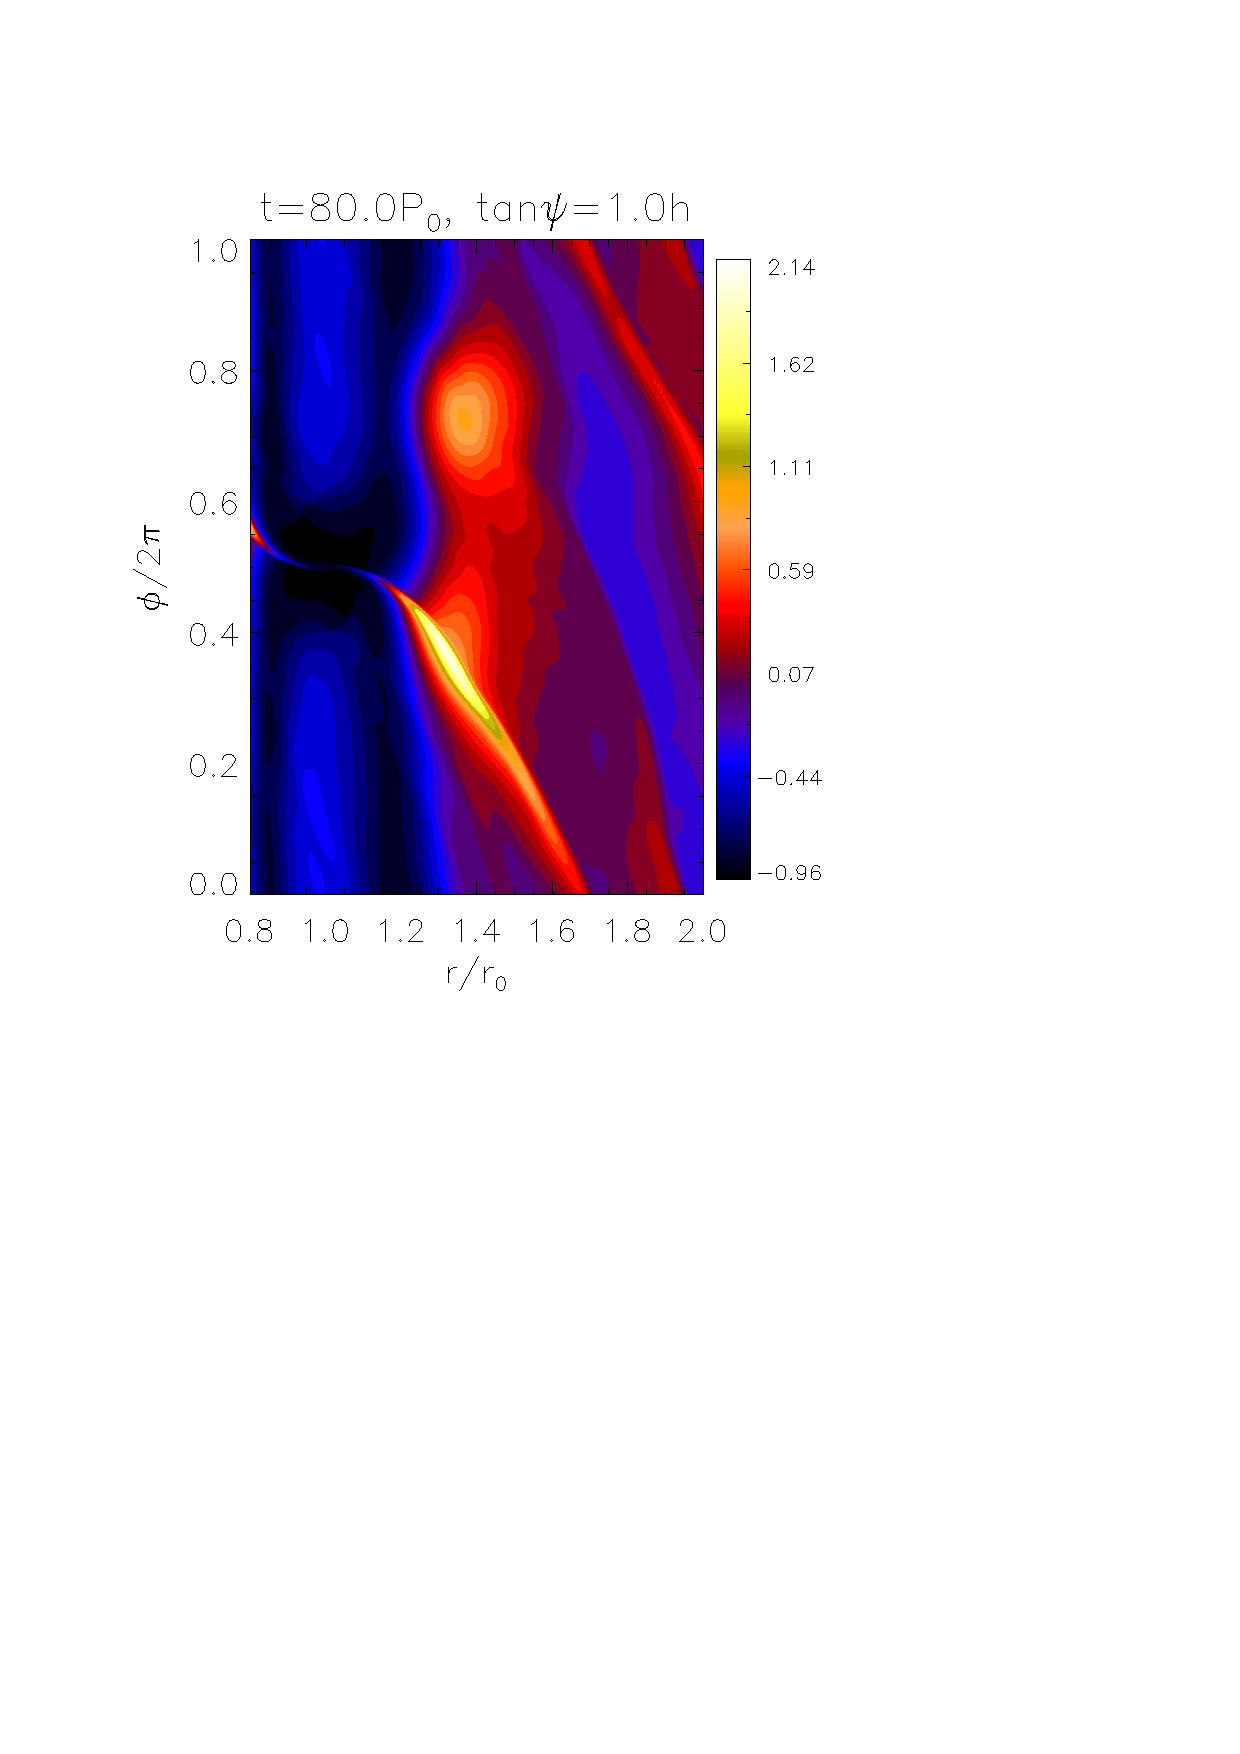
\includegraphics[scale=.27,clip=true,trim=2.3cm
     %% 1.84cm 0.cm
     %% 0.99cm]{figures/jup2_nuamp10_pdisk008}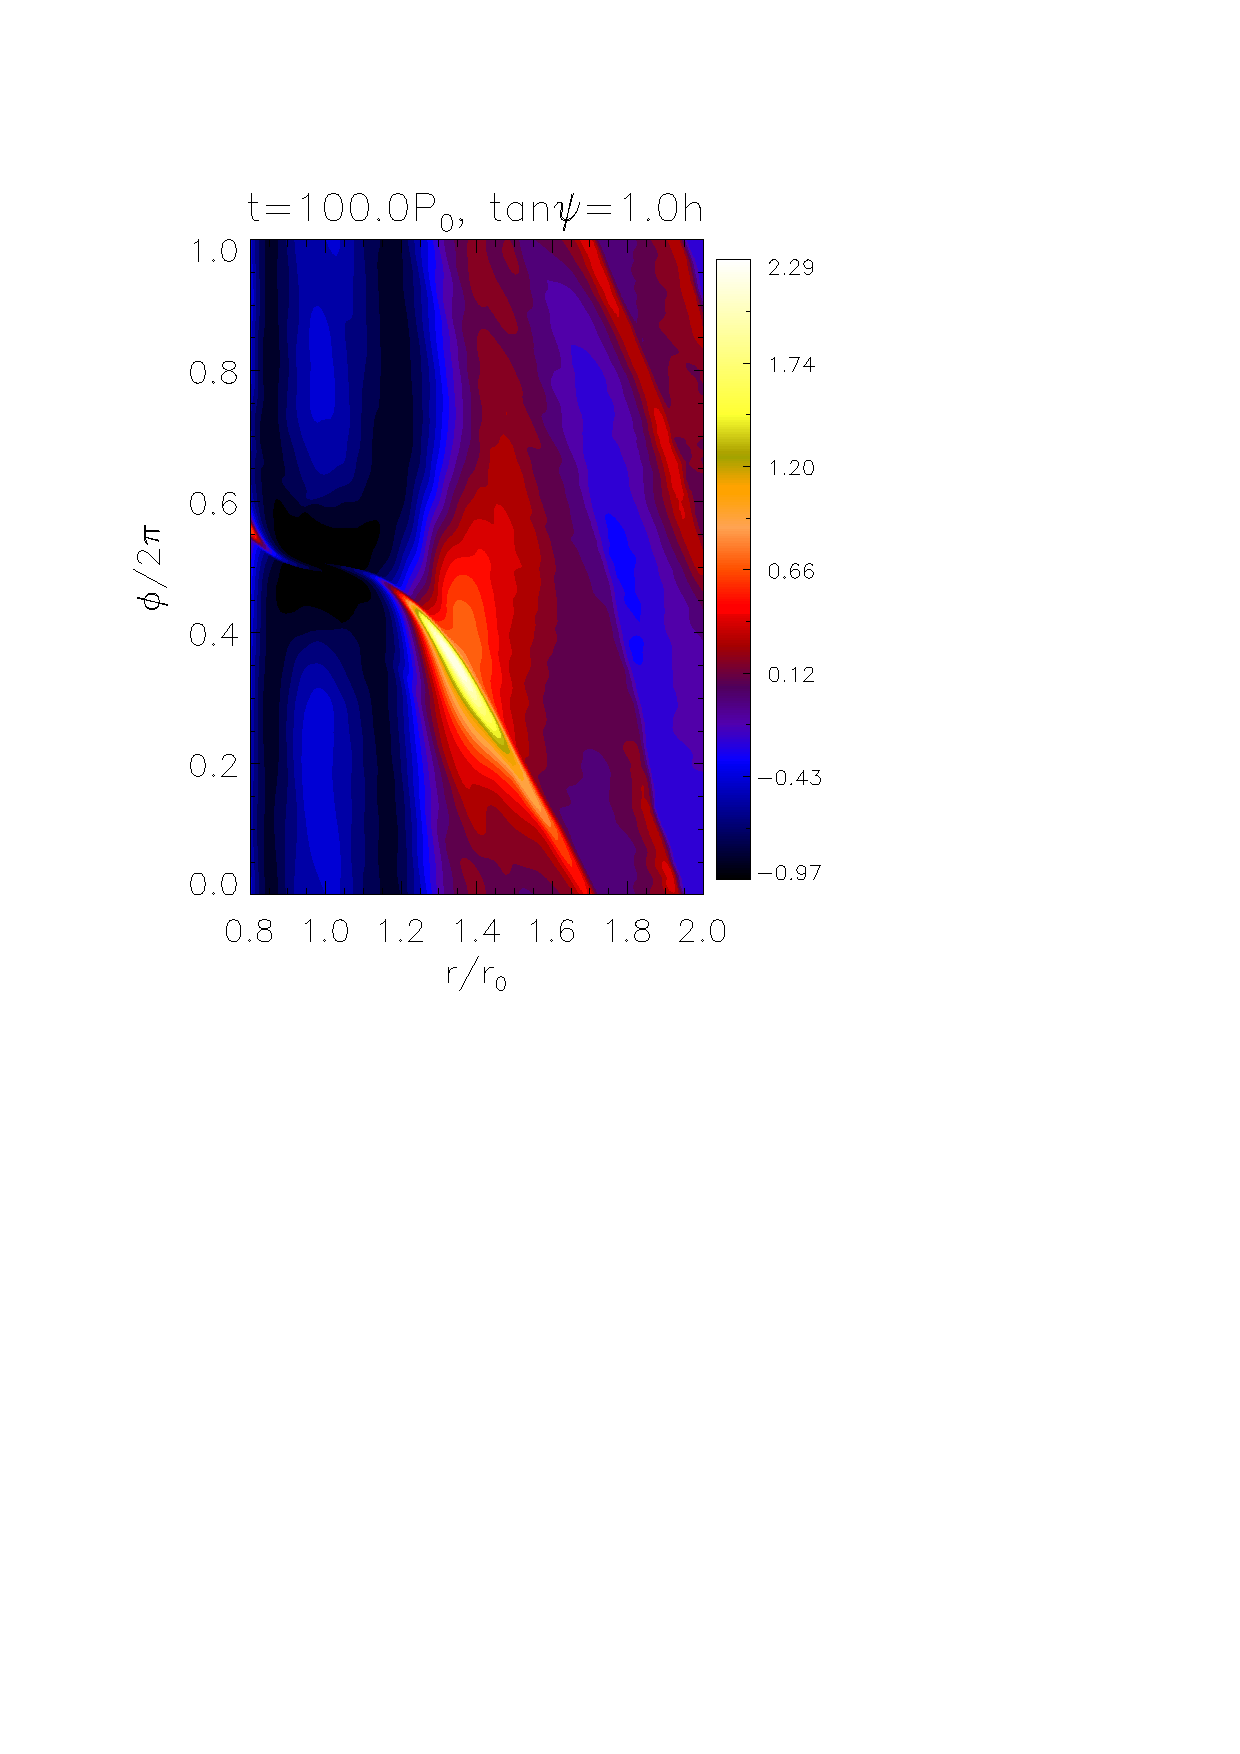
\includegraphics[scale=.27,clip=true,trim=2.3cm
     %% 1.84cm 0.cm
     %% 0.99cm]{figures/jup2_nuamp10_pdisk010}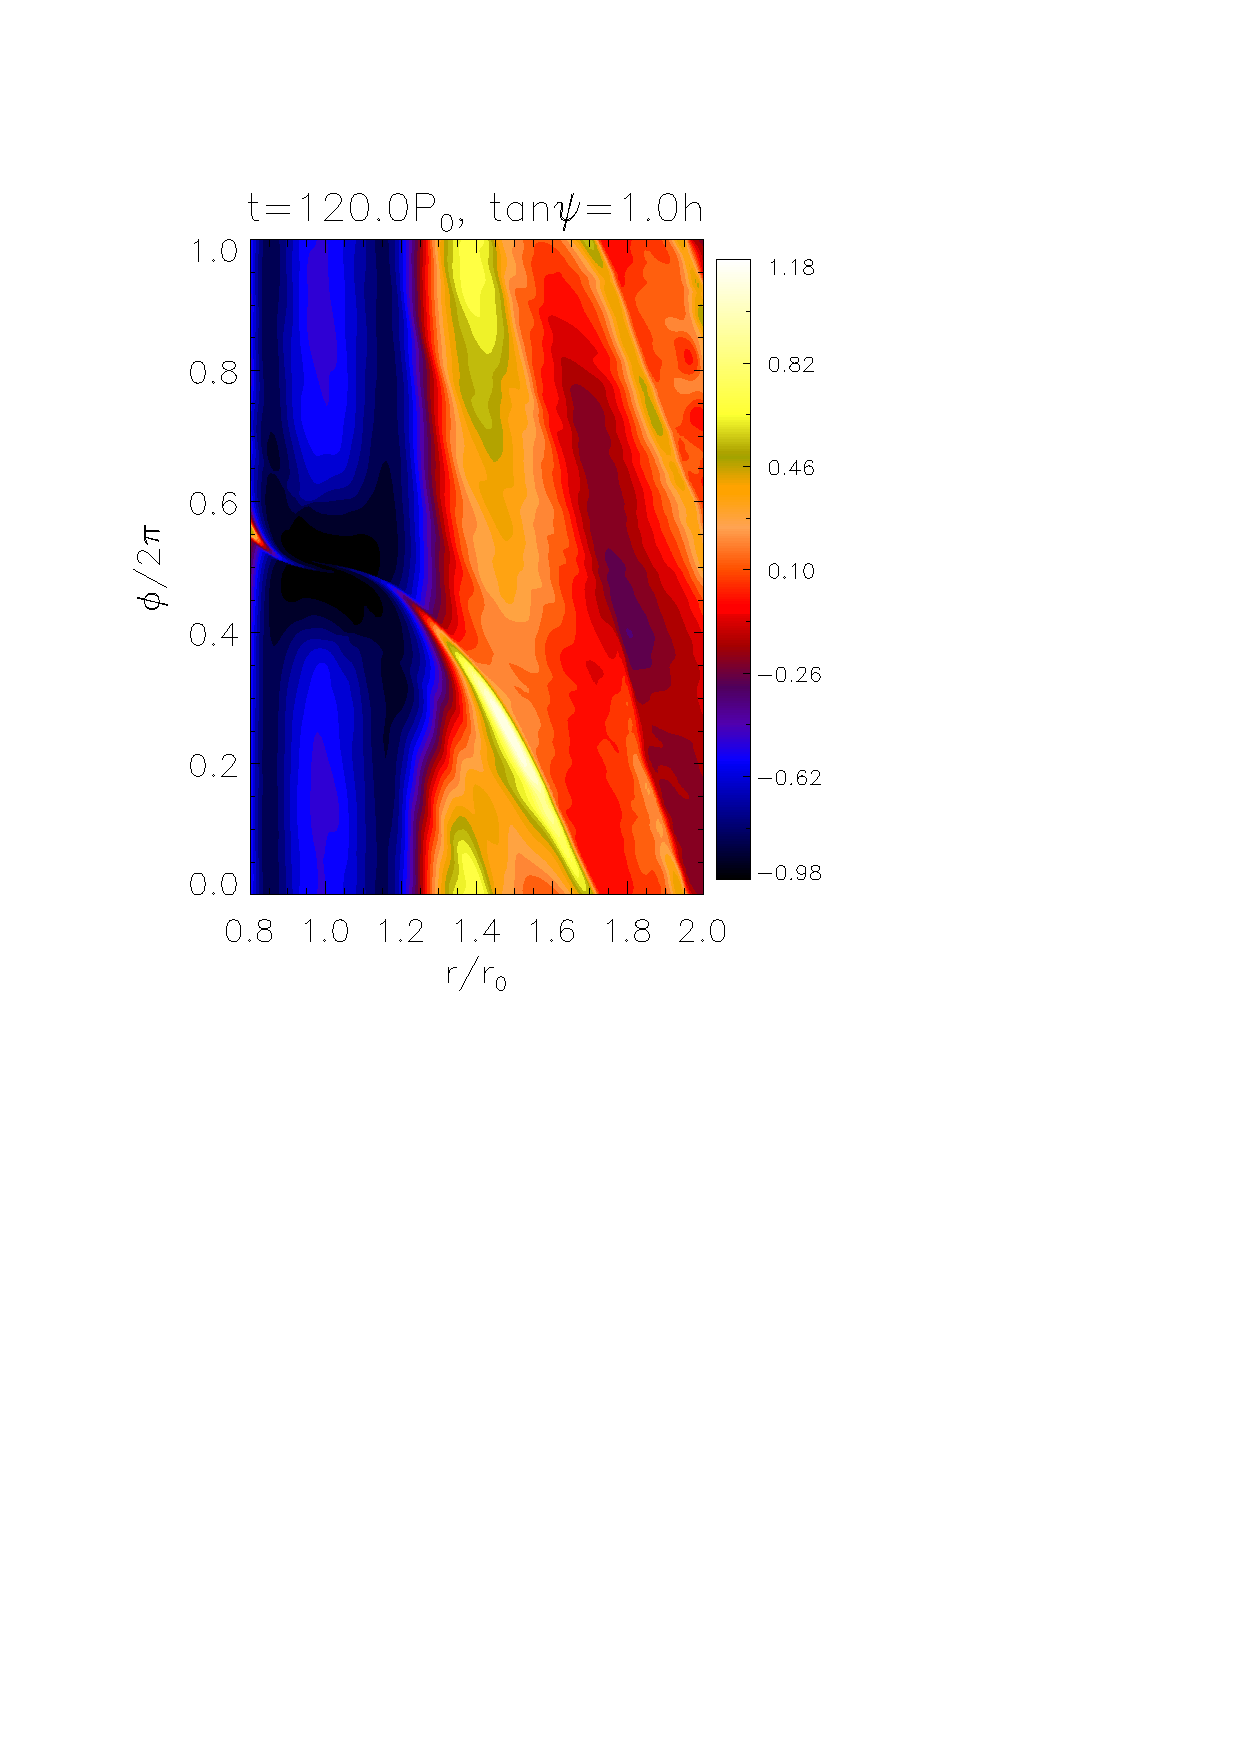
\includegraphics[scale=.27,clip=true,trim=2.3cm
     %% 1.84cm 0.cm
     %% 0.99cm]{figures/jup2_nuamp10_pdisk012}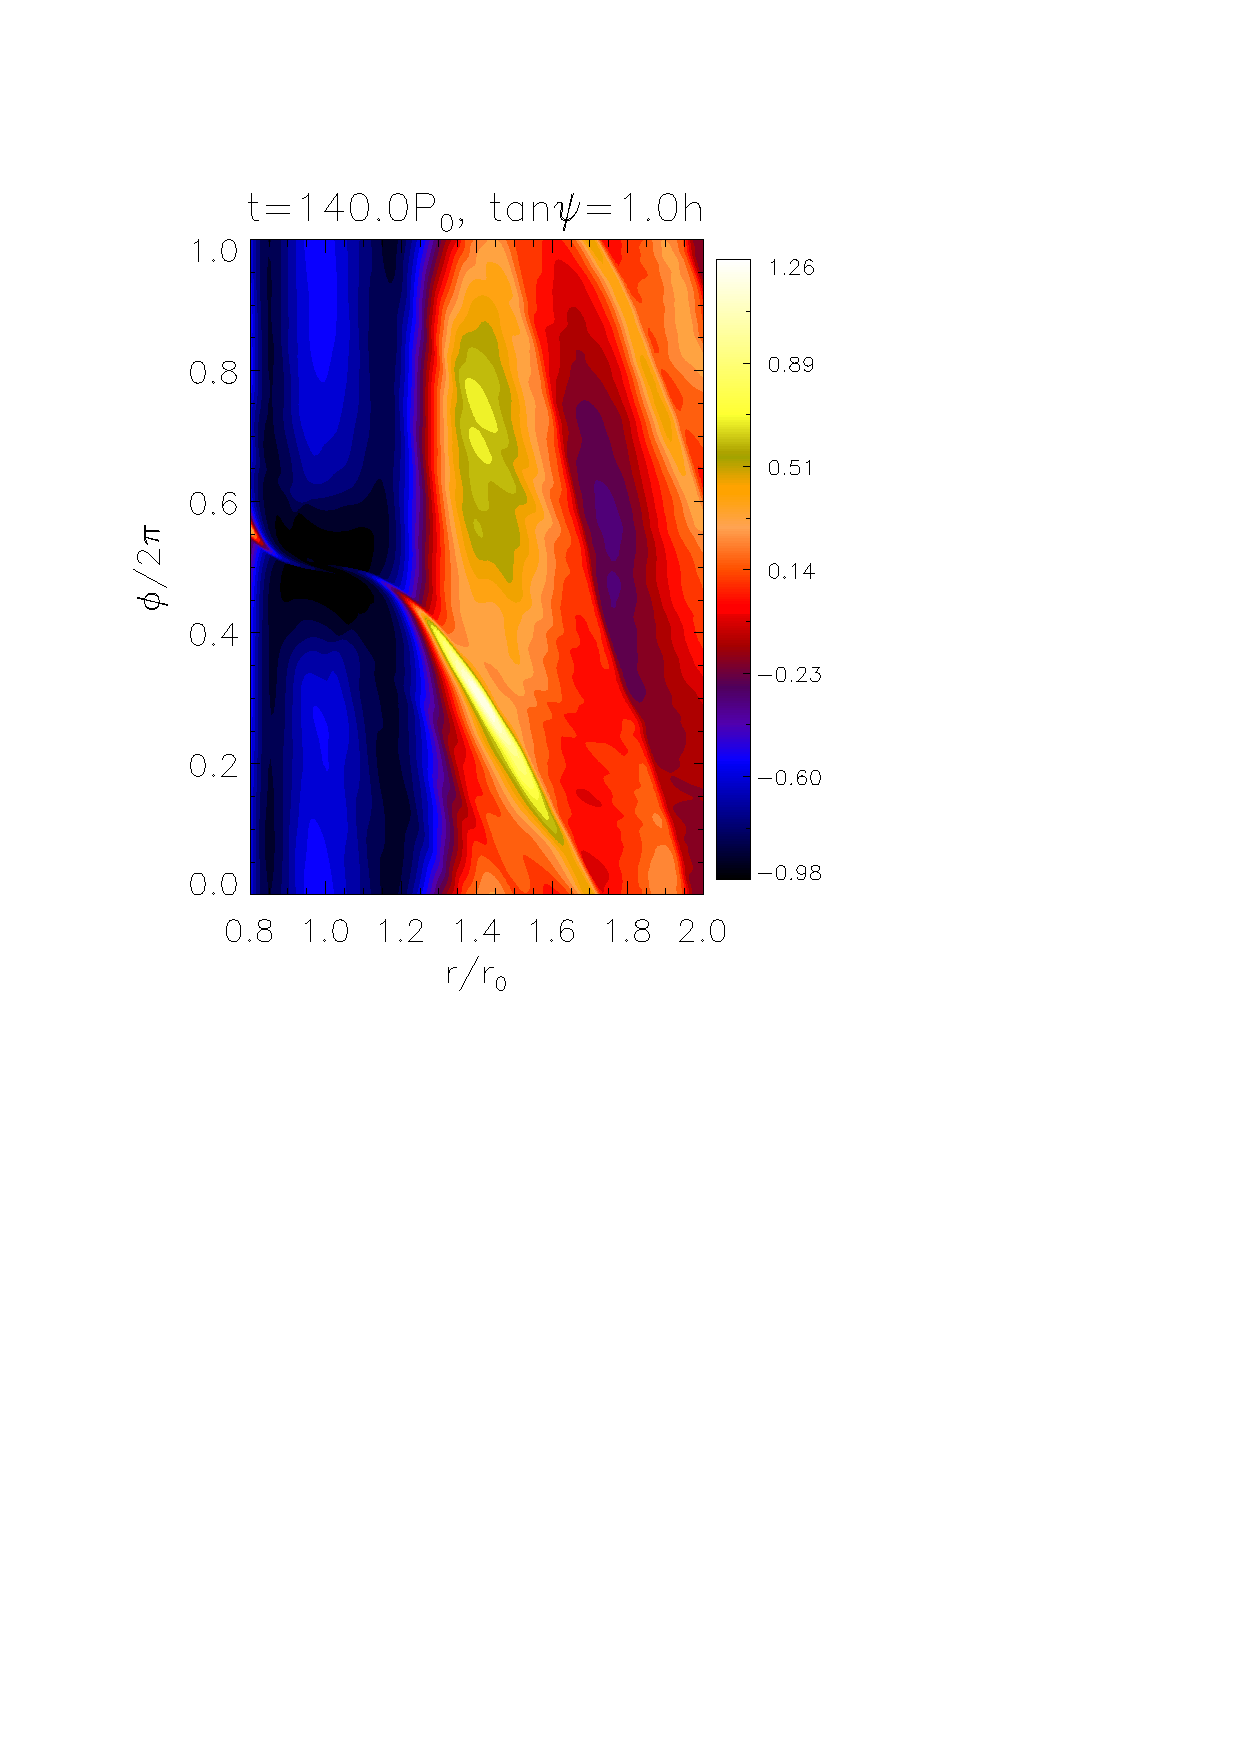
\includegraphics[scale=.27,clip=true,clip=true,trim=2.3cm
     %% 1.84cm 0.cm
     %% 0.99cm]{figures/jup2_nuamp10_pdisk014} \\
   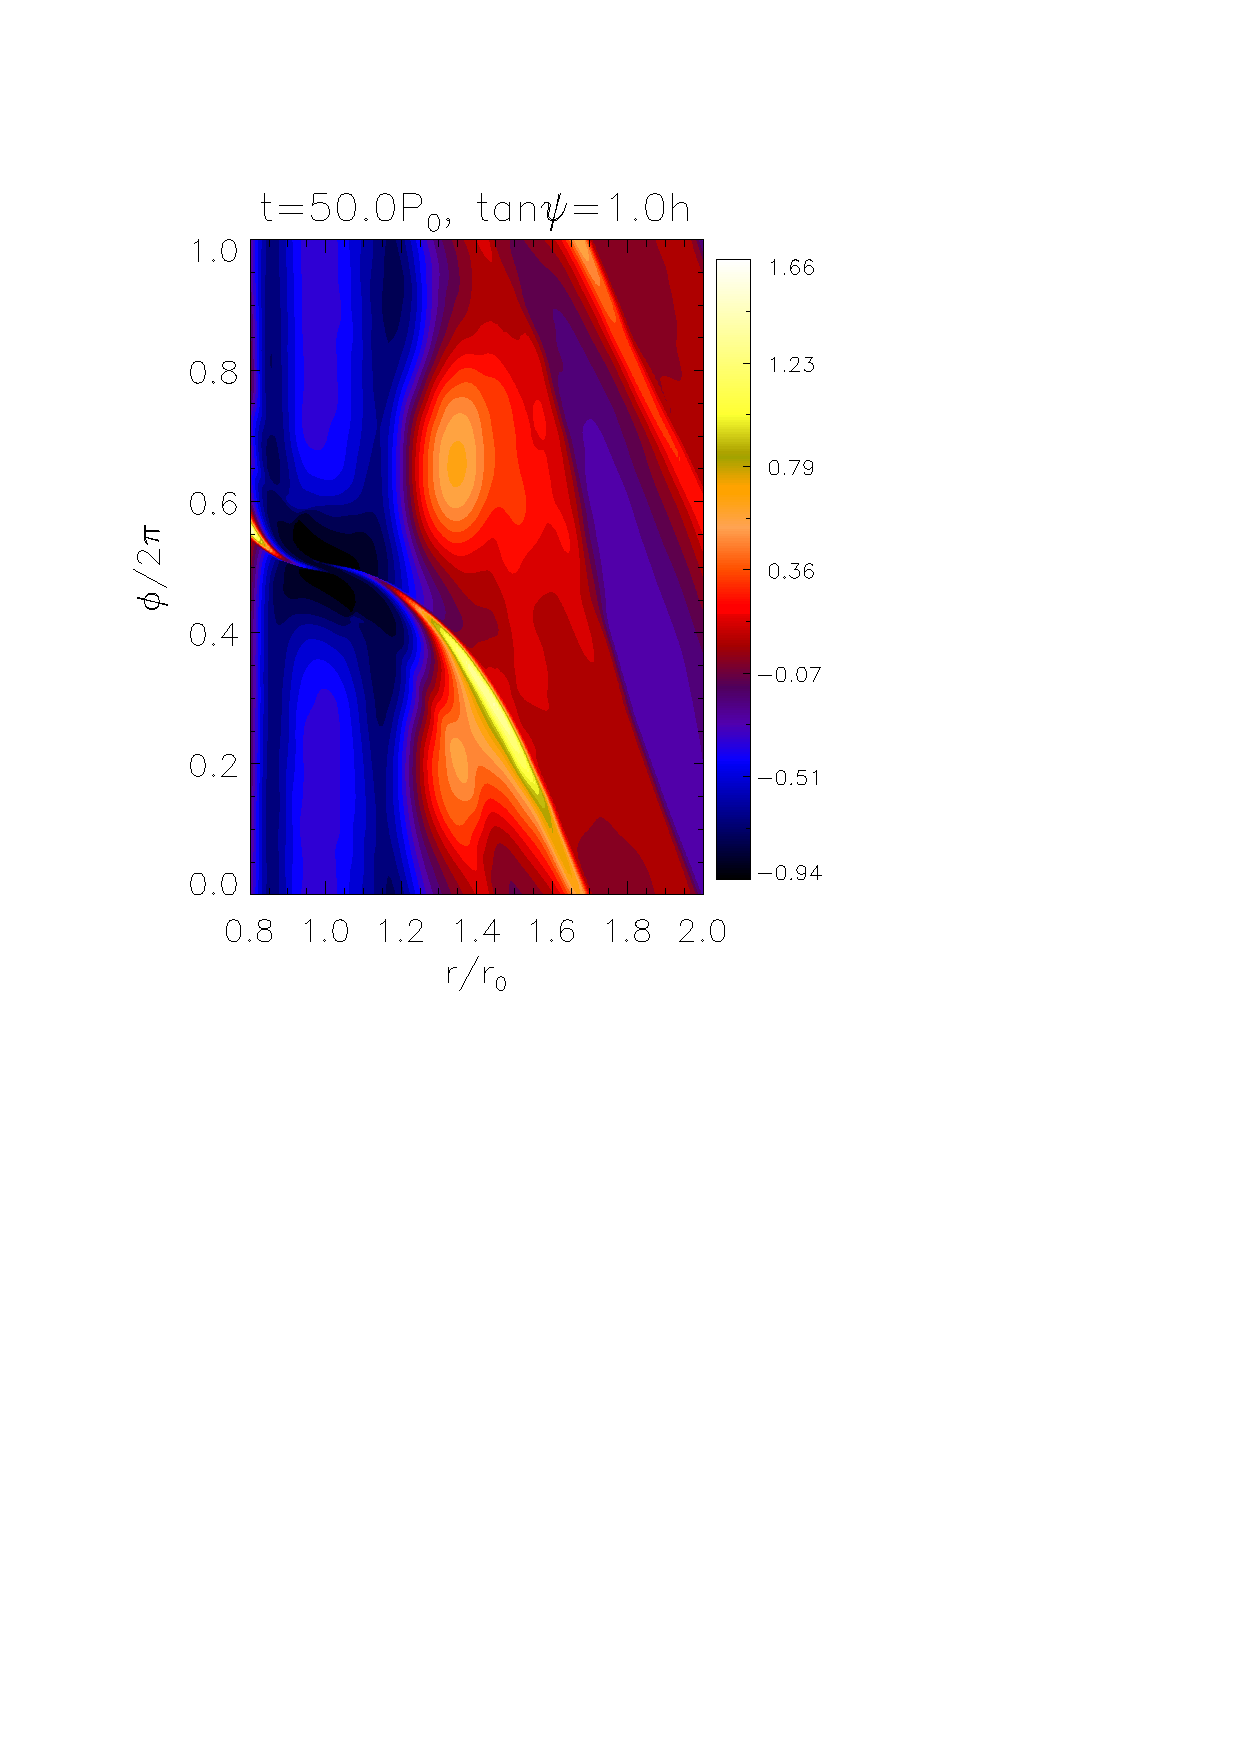
\includegraphics[scale=.39,clip=true,trim=0cm 0.cm 0.0cm
     0.99cm]{figures/jup3_nuamp10_pdisk005}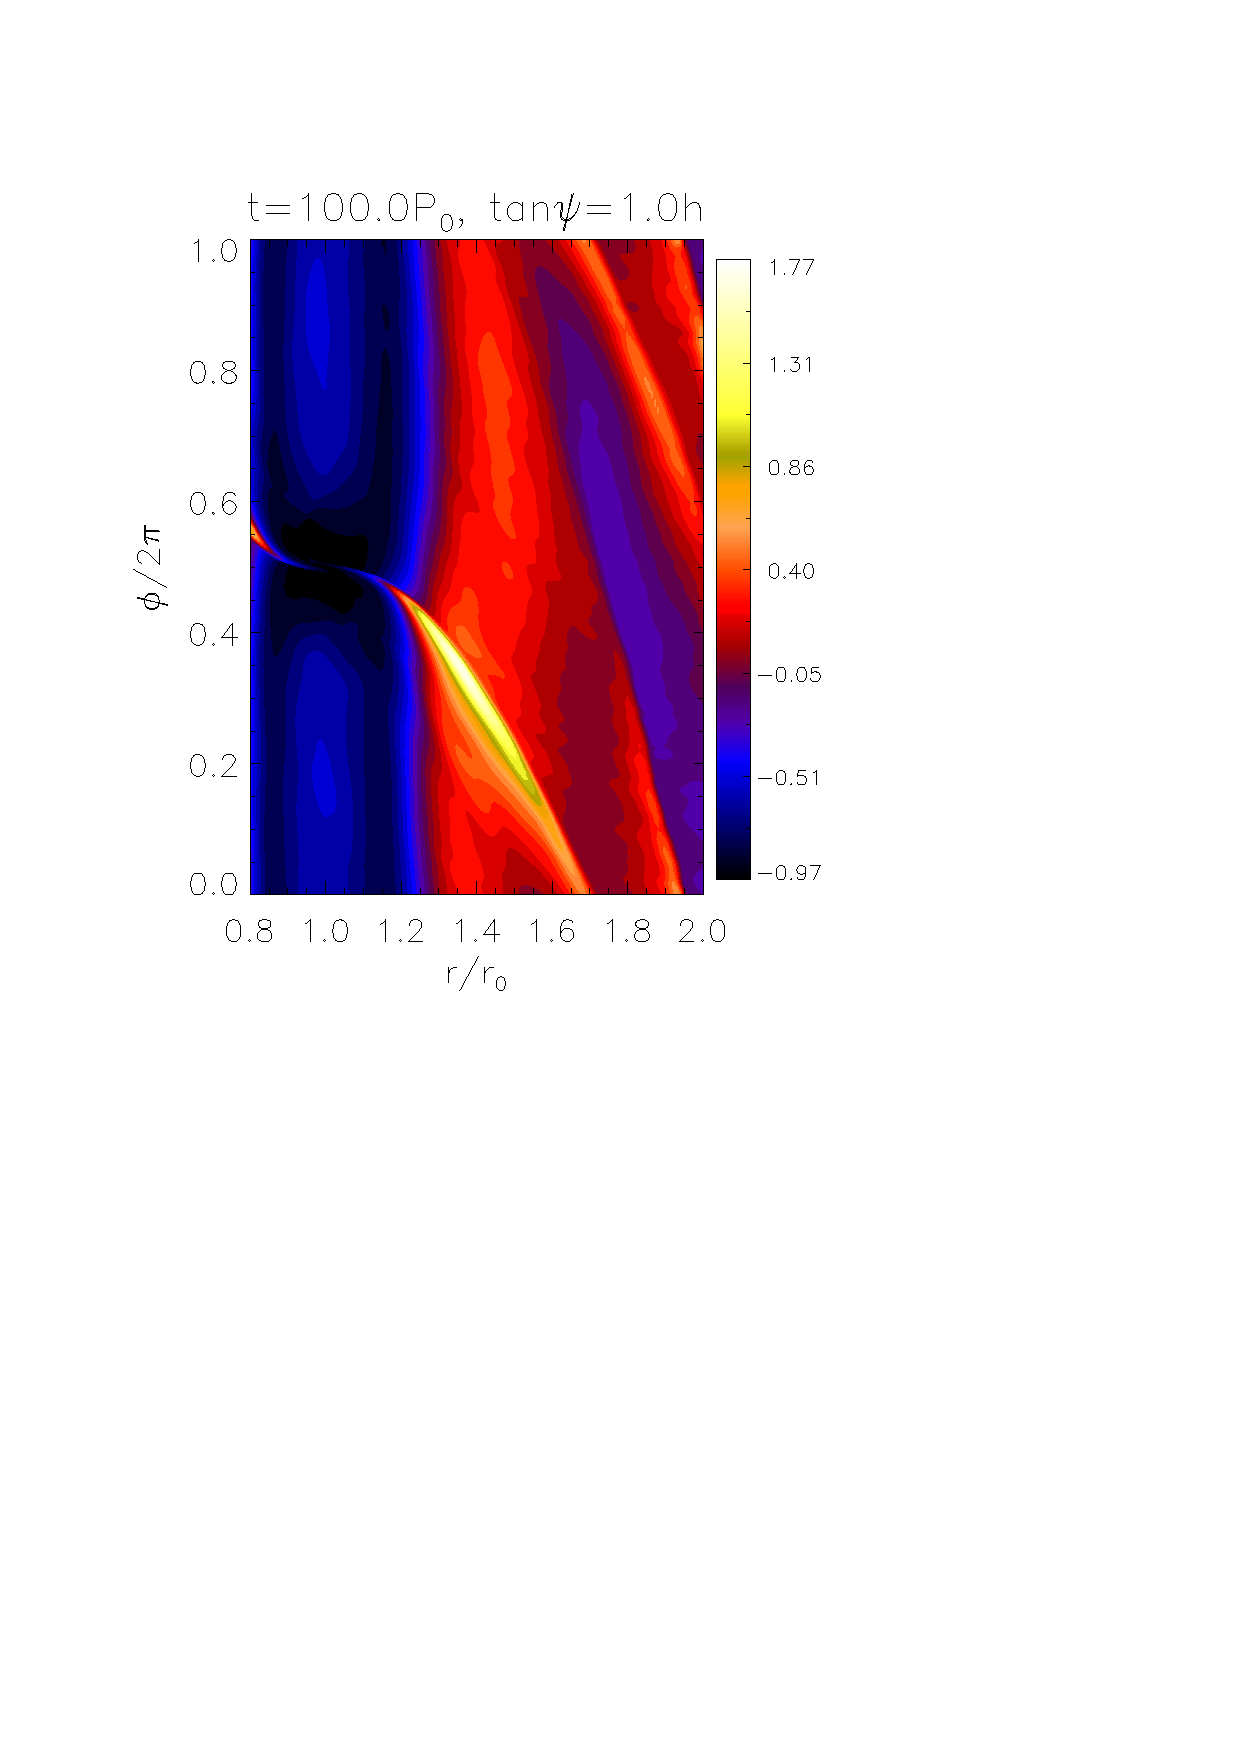
\includegraphics[scale=.39,clip=true,trim=2.3cm
     0.cm 0.cm
     0.99cm]{figures/jup3_nuamp10_pdisk010}\\%% 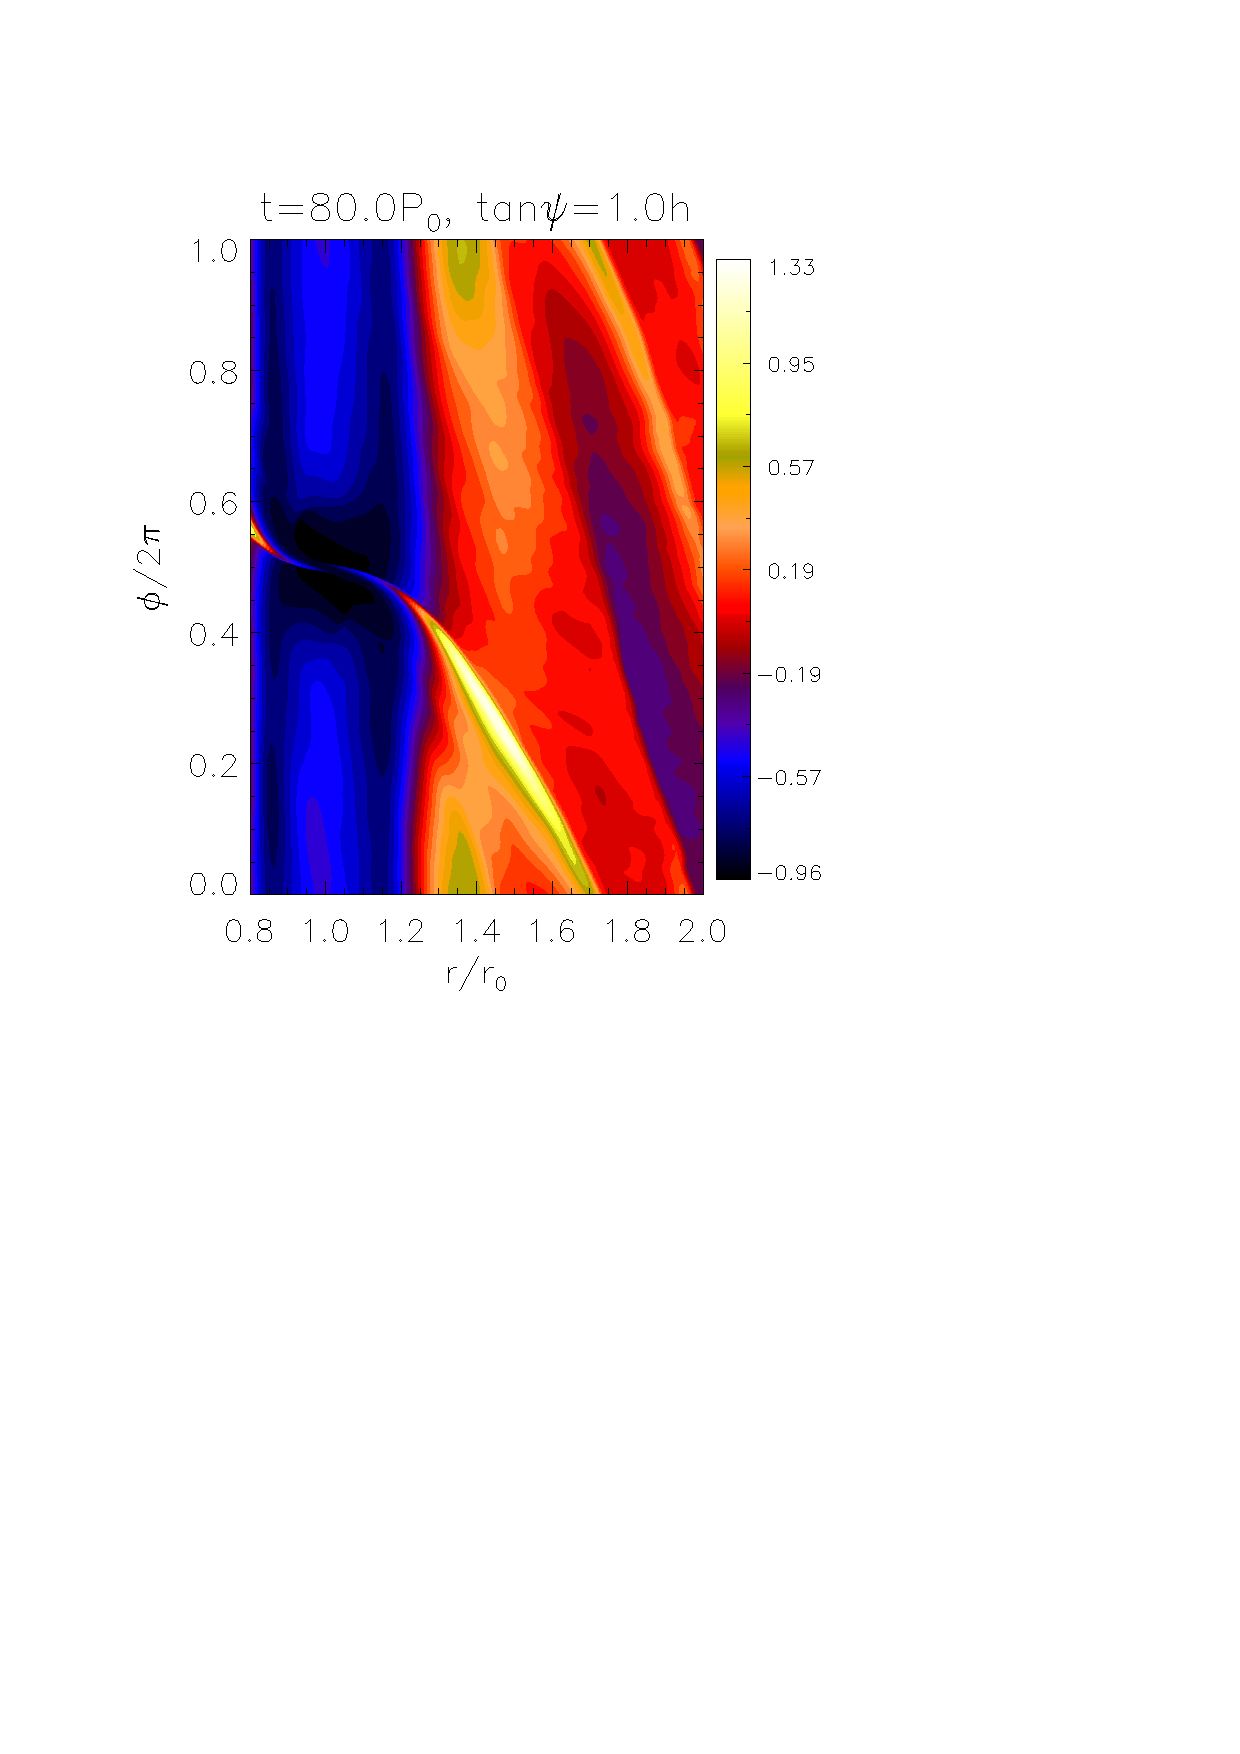
\includegraphics[scale=.27,clip=true,trim=2.3cm
     %% 0.cm 0.cm
     %% 0.99cm]{figures/jup3_nuamp10_pdisk008}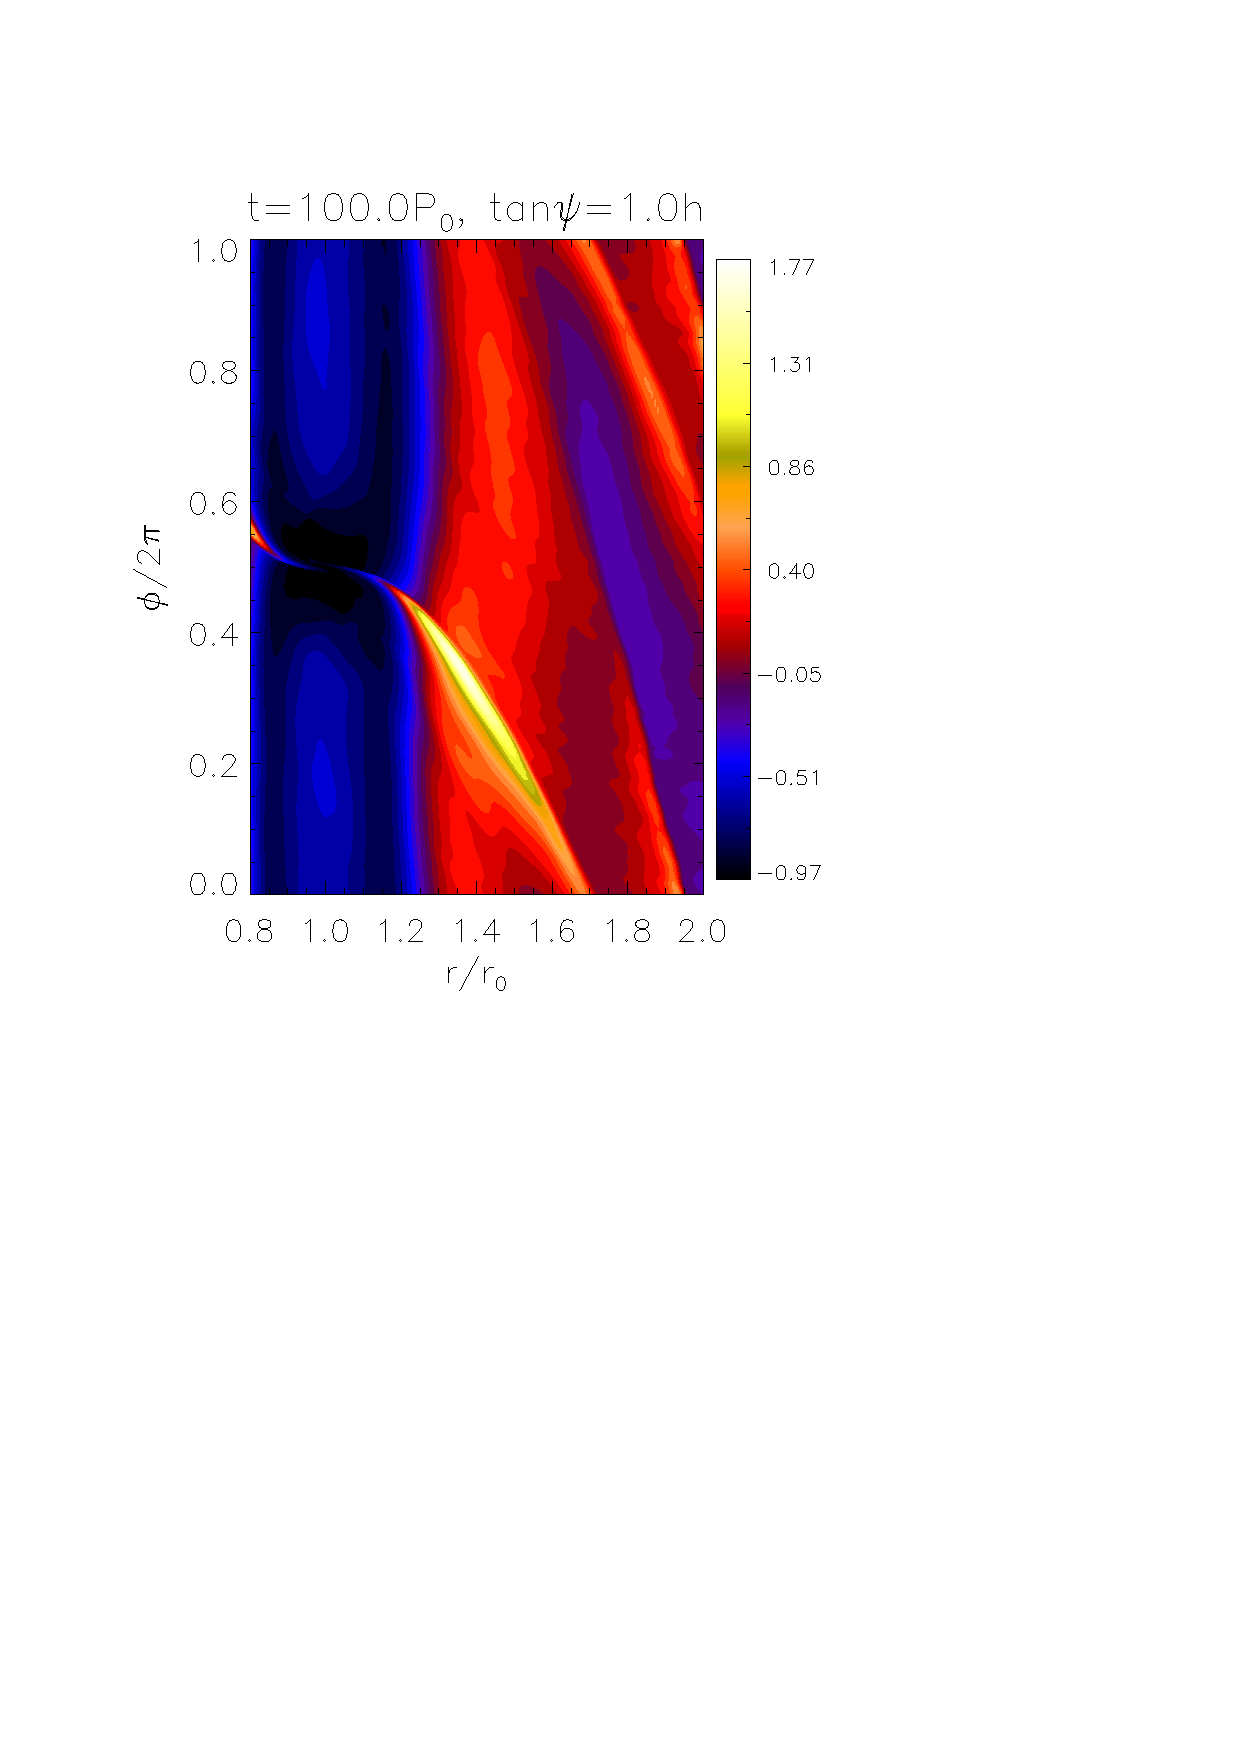
\includegraphics[scale=.27,clip=true,trim=2.3cm
     %% 0.cm 0.cm
     %% 0.99cm]{figures/jup3_nuamp10_pdisk010}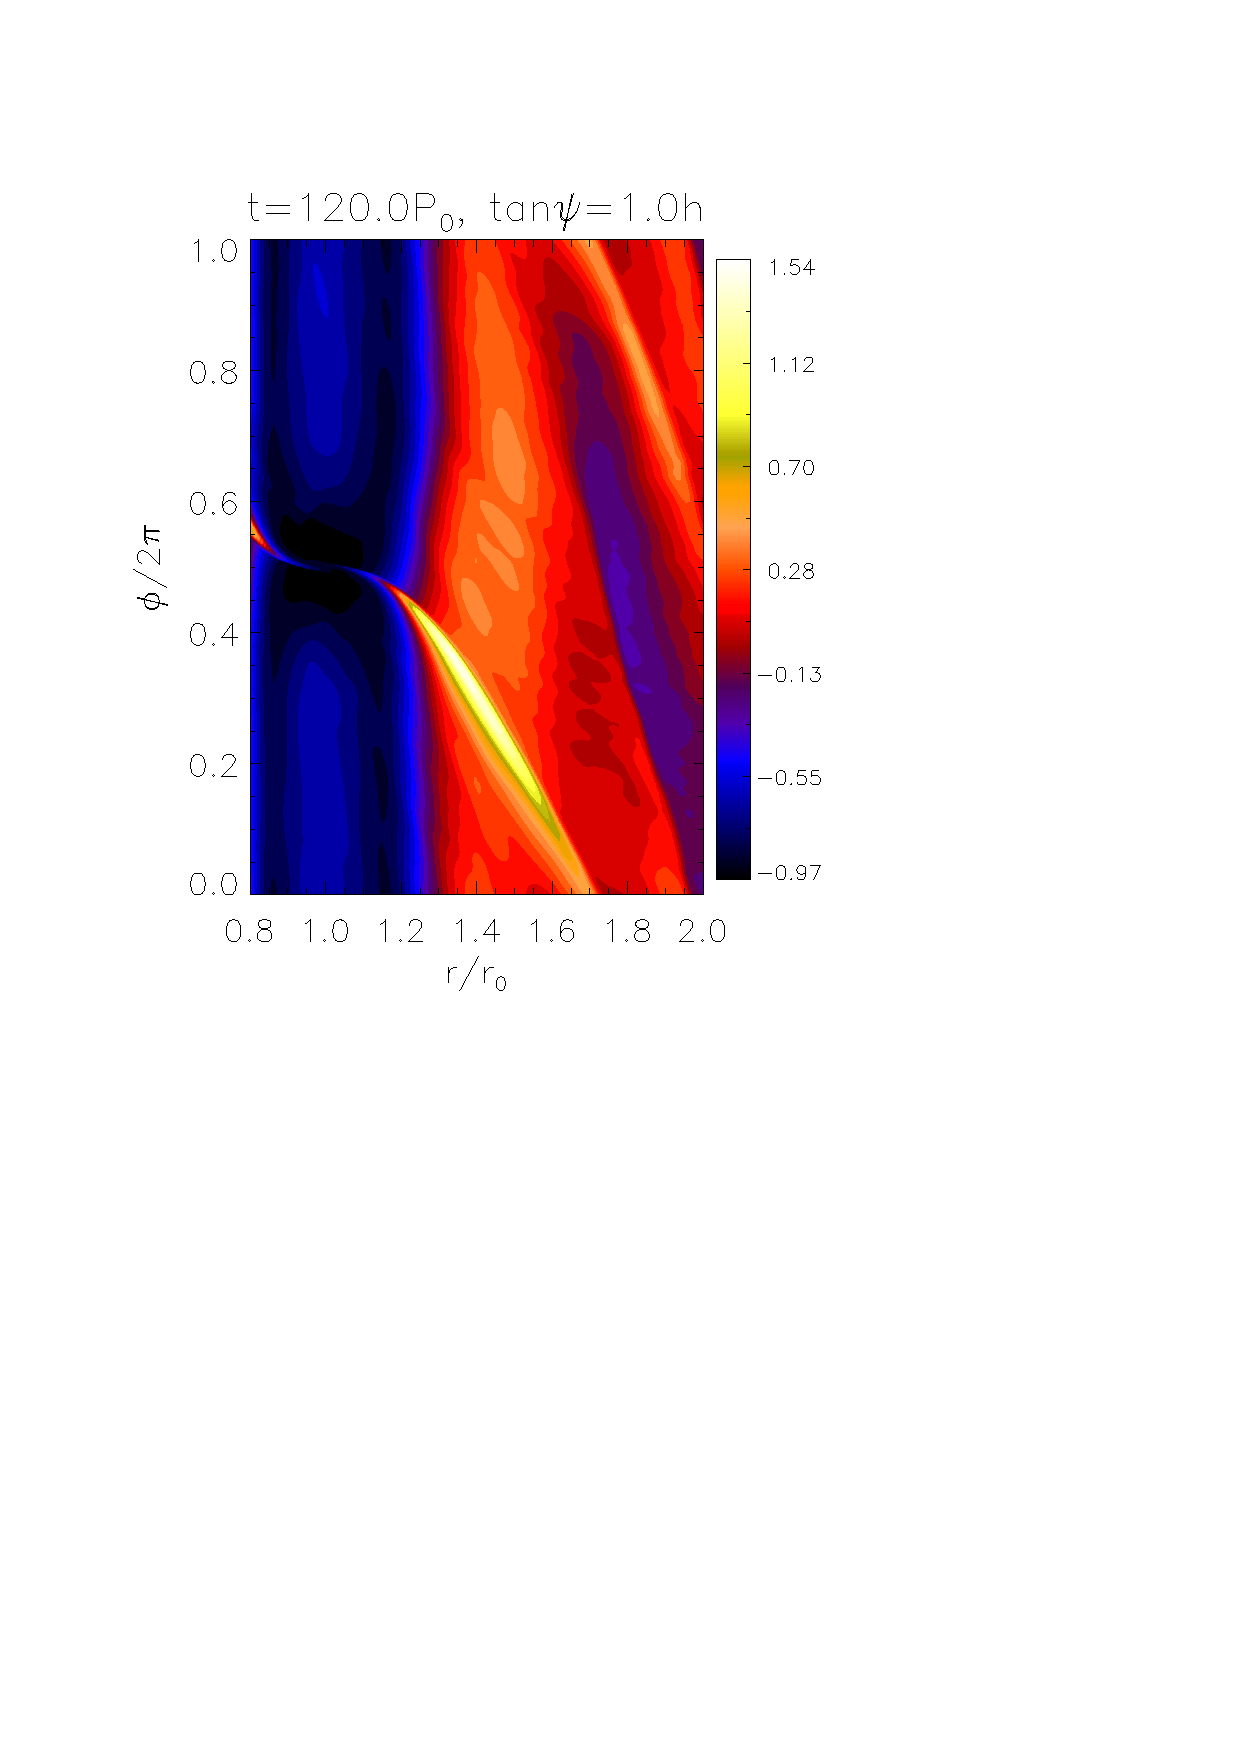
\includegraphics[scale=.27,clip=true,trim=2.3cm
     %% 0.cm 0.cm
     %% 0.99cm]{figures/jup3_nuamp10_pdisk012}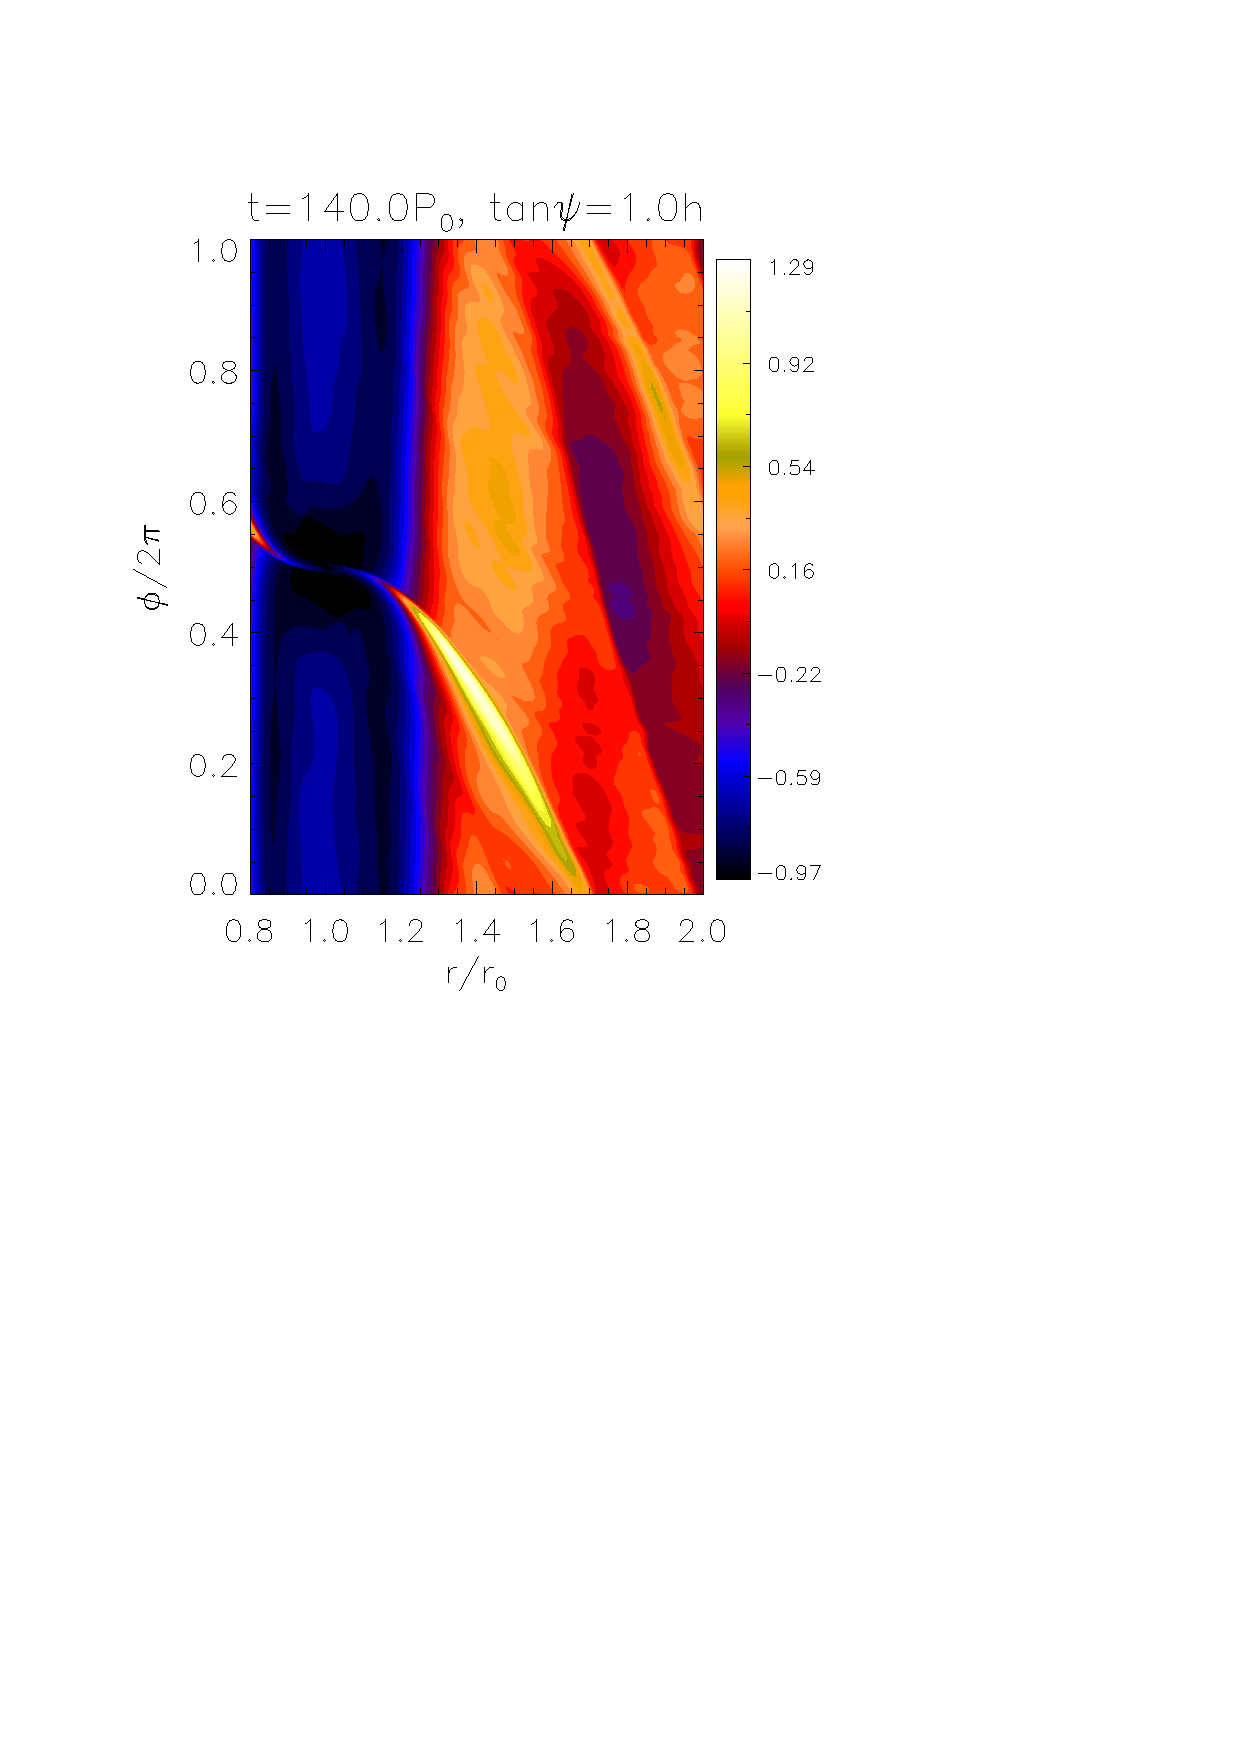
\includegraphics[scale=.27,clip=true,clip=true,trim=2.3cm
     %% 0.cm 0.cm
     %% 0.99cm]{figures/jup3_nuamp10_pdisk014} \\
   \caption{Density perturbation $\delta\rho$ for disc-planet
     simulations case P0 (top), P1 (middle) and P2 (bottom). The
     thickness of the viscous layer occupies $0\%,\,25\%$ and $50\%$
     of the uppermost vertical domain from top to bottom. 
   \label{jup0}}
 \end{figure}


\subsubsection{Diffusion of potential vorticity}
It is instructive to examine the PV evolution for the above cases 
because the RWI is associated with PV minima. We compare the 
azimuthally averaged PV profiles in Fig. \ref{planet_gap_PV}.  

At early times ($t\lesssim50P_0$) all three cases have similar PV
profiles, namely a minima at the outer gap edge ($R\simeq1.3r_0$), and
all cases at this stage develops the $m=2$ RWI. Therefore layered
viscosity is insignificant on short timescales, consistent with the
fact that the linear RWI operates on dynamical timescales which is
shorter than local viscous timescales. 

Viscosity takes effect at late times ($t\gtrsim100P_0$). It is clear
from Fig. \ref{planet_gap_PV} that the outer gap edge PV minimum
becomes more blunt with respect to time and the thickness of the
viscous layer. Thus a viscous layer has a global effect in the
vertical direction. 

Notice the PV maxima grows over the course of the simulation, but at
a slower rate as the viscous layer is thickened. By $t=150P_0$ the
outer PV maximum in case P0 is almost 3 times larger than that in case
P3. Although PV maxima remains stable in non-self-gravitating
discs \citep{lin11a}, but one might consider a more sharply peaked PV
maximum makes the adjacent PV minimum relatively deeper. In other
words the PV maxima helps to trap the unstable vortex modes. 
This may explain why the vortex in case P0 is sustained, while that in
case P3 does not survive: vorticity is being effectively generated by
the planet in the former case where diffusion is unimportant.  

\begin{figure}
  \centering
  \includegraphics[width=\linewidth,clip=true,trim=0cm 1.66cm 0cm
    0.6cm]{figures/pdisk_vorten1d_cases_005.ps}\\\includegraphics[width=\linewidth,clip=true,trim=0cm
    1.66cm 0cm
    0.6cm]{figures/pdisk_vorten1d_cases_010.ps}\\\includegraphics[width=\linewidth,clip=true,trim=0cm
    0cm 0cm 0.6cm]{figures/pdisk_vorten1d_cases_015.ps} 
  \caption{Azimuthally averaged PV evolution for the two vertical
    scale-height disc-planet simulations. 
    \label{planet_gap_PV}}
\end{figure}

\subsubsection{Kinetic energy evolution}




\subsection{Viscous atmosphere}
%We now consider appending a viscous layer on top of the fiducial 
%case P0. 
Case P3 is the same as case P0 above, except with an increased
vertical domain size of $3H$ at the reference radius. Case P4 has a high-viscosity layer with
$\hat{\nu}\sim10^{-4}$ in the the uppermost scale-height of the
computational domain. In other words, the bulk of the 
%% has a viscosity $\hat{\nu} \sim 10^{-5}$ and $\hat{\nu}\sim 10^{-4}$
%% for cases P3 and P4, respectively. 
disk for case P4 has a low-viscosity of $\hat{\nu}\sim10^{-6}$, but
with a viscous atmosphere appended on top.  

Fig. \ref{jup0_3h} shows the density pertubation at $t=100P_0$ for
cases P3 and P4. Case P3 is essentially identical to case P0, so the 
vortex instability is not affected by vertical domain size. We note
that the viscosity is increased in the disc atmosphere, where the
density is a factor $\sim 7$ times smaller than the midplane (but the
viscosity is $100$ times larger). The viscous layer has surpressed
vortex formation. This implies that vortex formation via
the RWI at planetary gap edges can not tolerate a signigicantly
viscous atmosphere, even if such a layer only occurs away from the
midplane.    

\begin{figure}
   \centering
   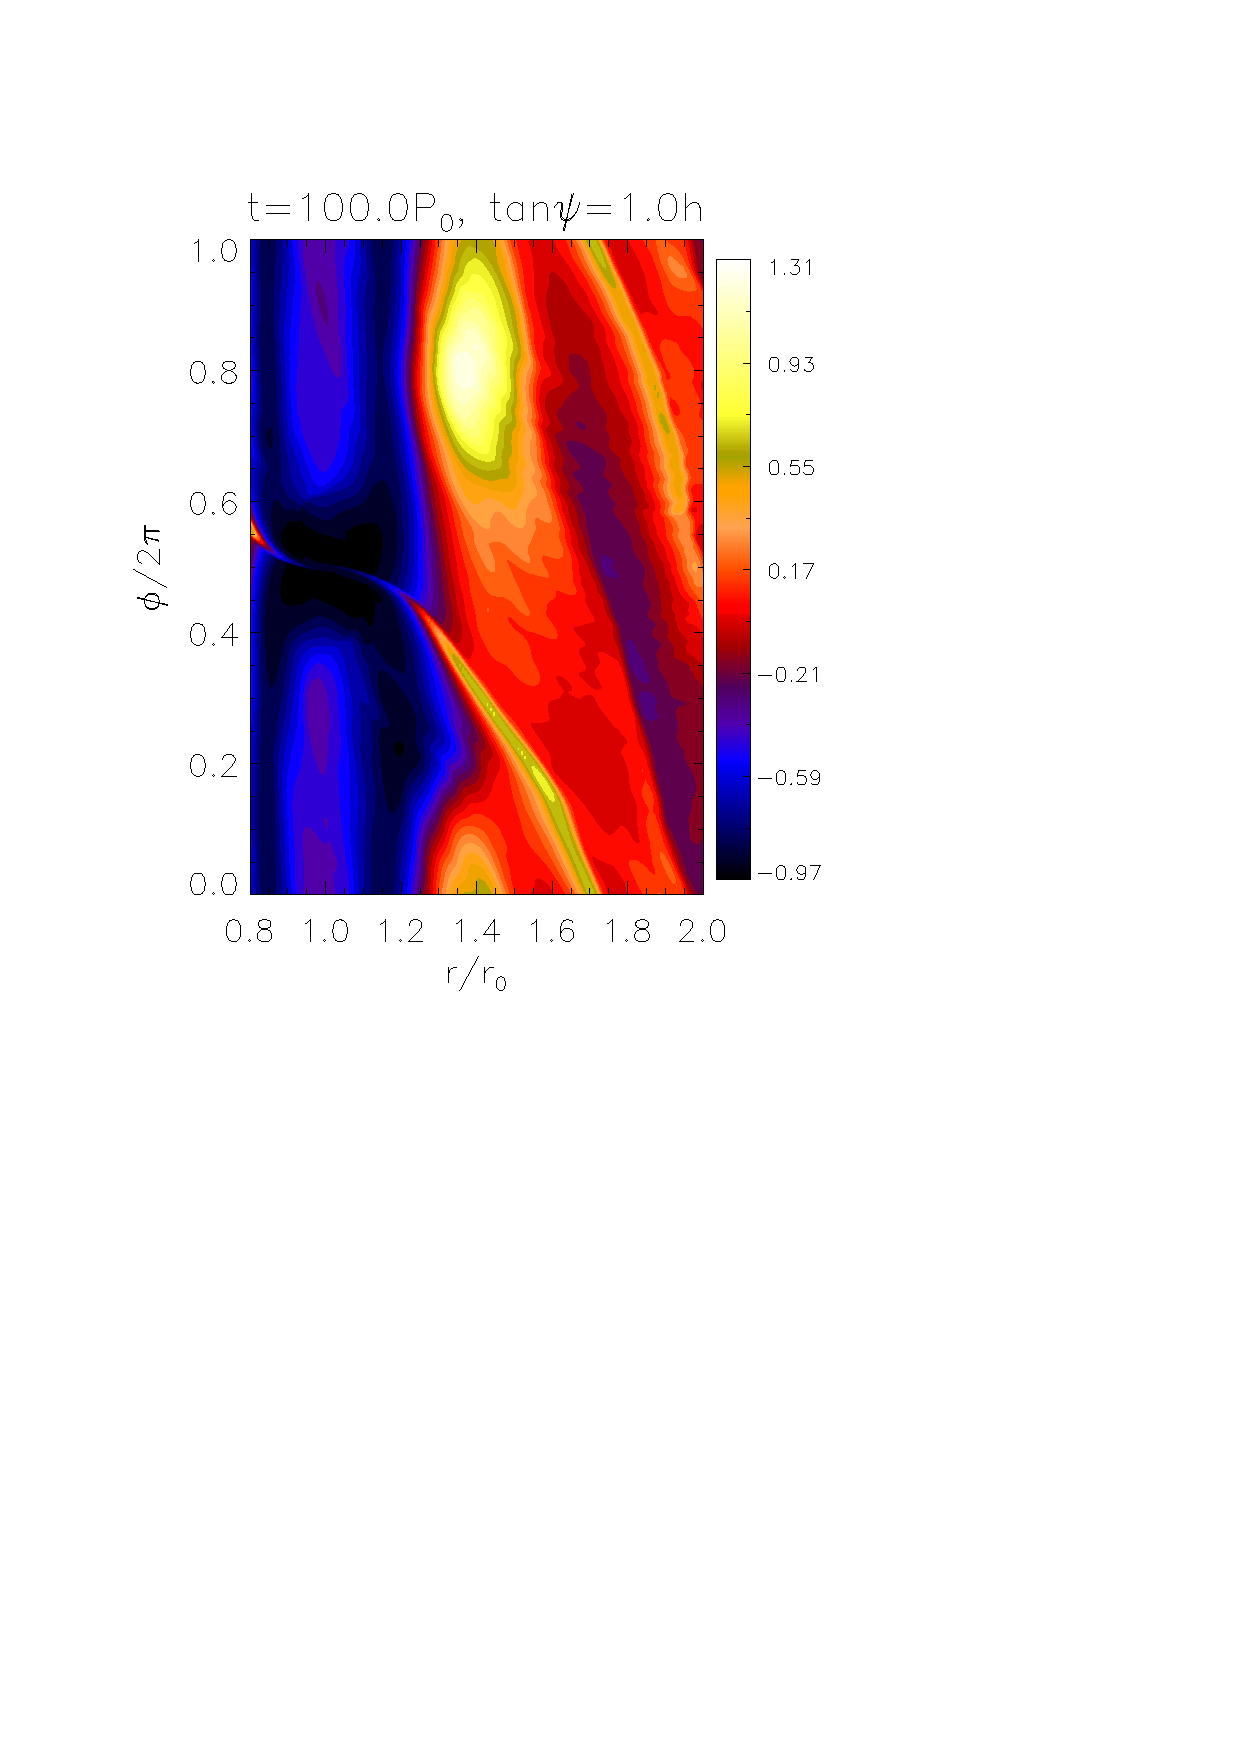
\includegraphics[scale=.39,clip=true,trim=0cm 1.84cm 0cm
     0cm]{figures/jup0_3h_pdisk010}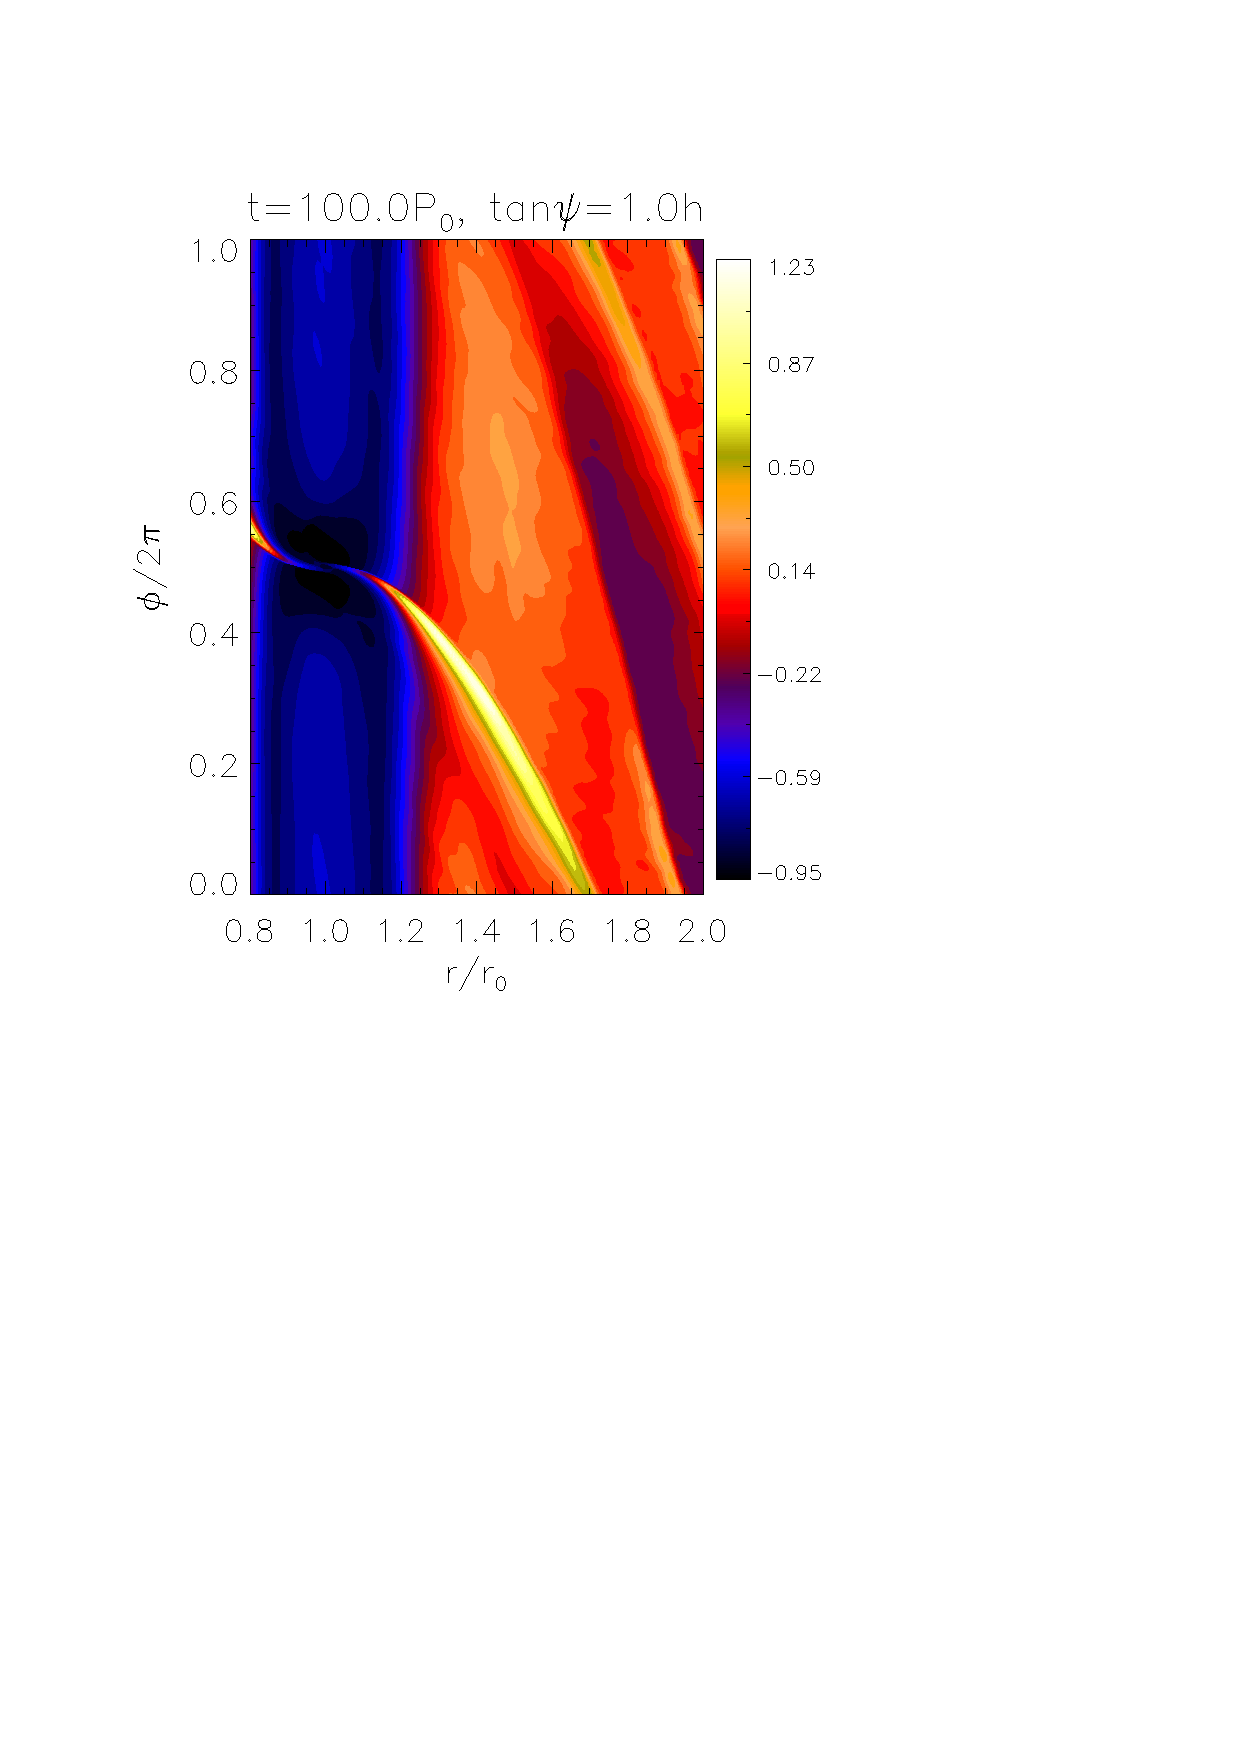
\includegraphics[scale=.39,clip=true,trim=2.3cm
     1.84cm 0cm
     0cm]{figures/jup1_3h_pdisk008}
   \caption{Density perturbation $\delta\rho$ at the end of the
     disc-planet simulations case P3 (left, no viscous layer) and P4
     (right, viscous layer occupies $33\%$ of the uppermost vertical
     domain).   
     \label{jup0_3h}}
\end{figure}
 


%\subsection{Locally isothermal simulations}
